% !TeX root = ../../main_socg.tex

In this section we will discuss a number of experiments which illustrate the benefit of truncated diagrams, and their approximation by relative diagrams, in comparison to their restricted counterparts.
We will focus on the persistent homology of functions on a square 2d grid.%---that is, functions with non-trivial persistent homology in dimensions zero and one.
% While these experiments can be conducted in dimension zero or one we will focus on $\hom_1$.
We chose as our function a radially symmetric damped sinusoid with random noise, depicted in Figure~\ref{fig:ripple1}, as it has prominent persistent homology in dimension one.

\paragraph*{Experimental setup.}

\begin{figure}[htbp]
  \centering
  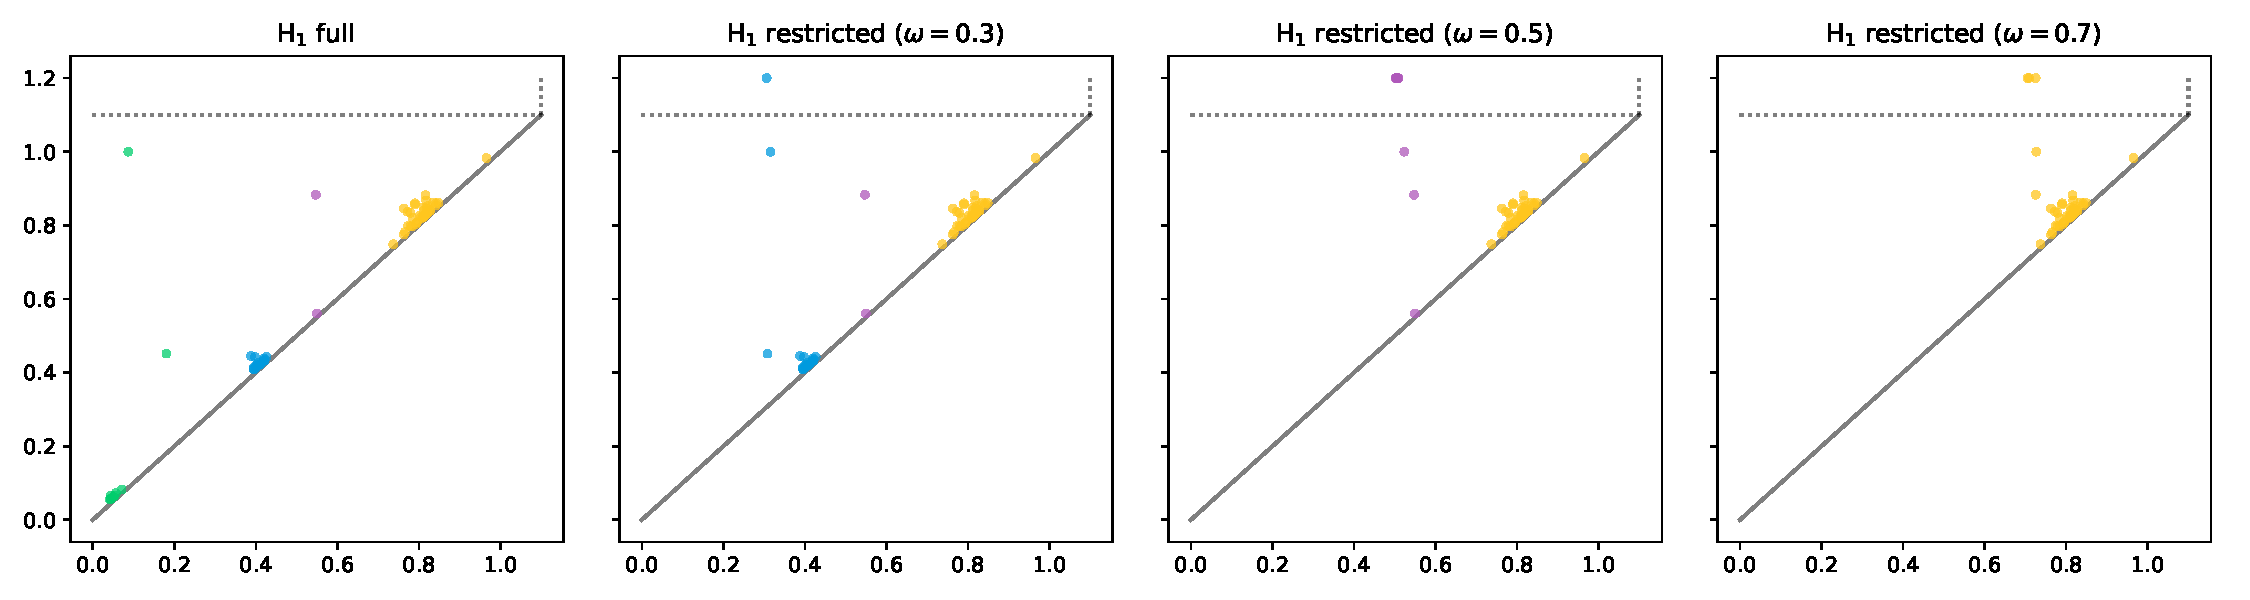
\includegraphics[trim=0 0 790 0, clip, width=0.3\textwidth]{scripts/figures/matching2/full-dgm.pdf}
  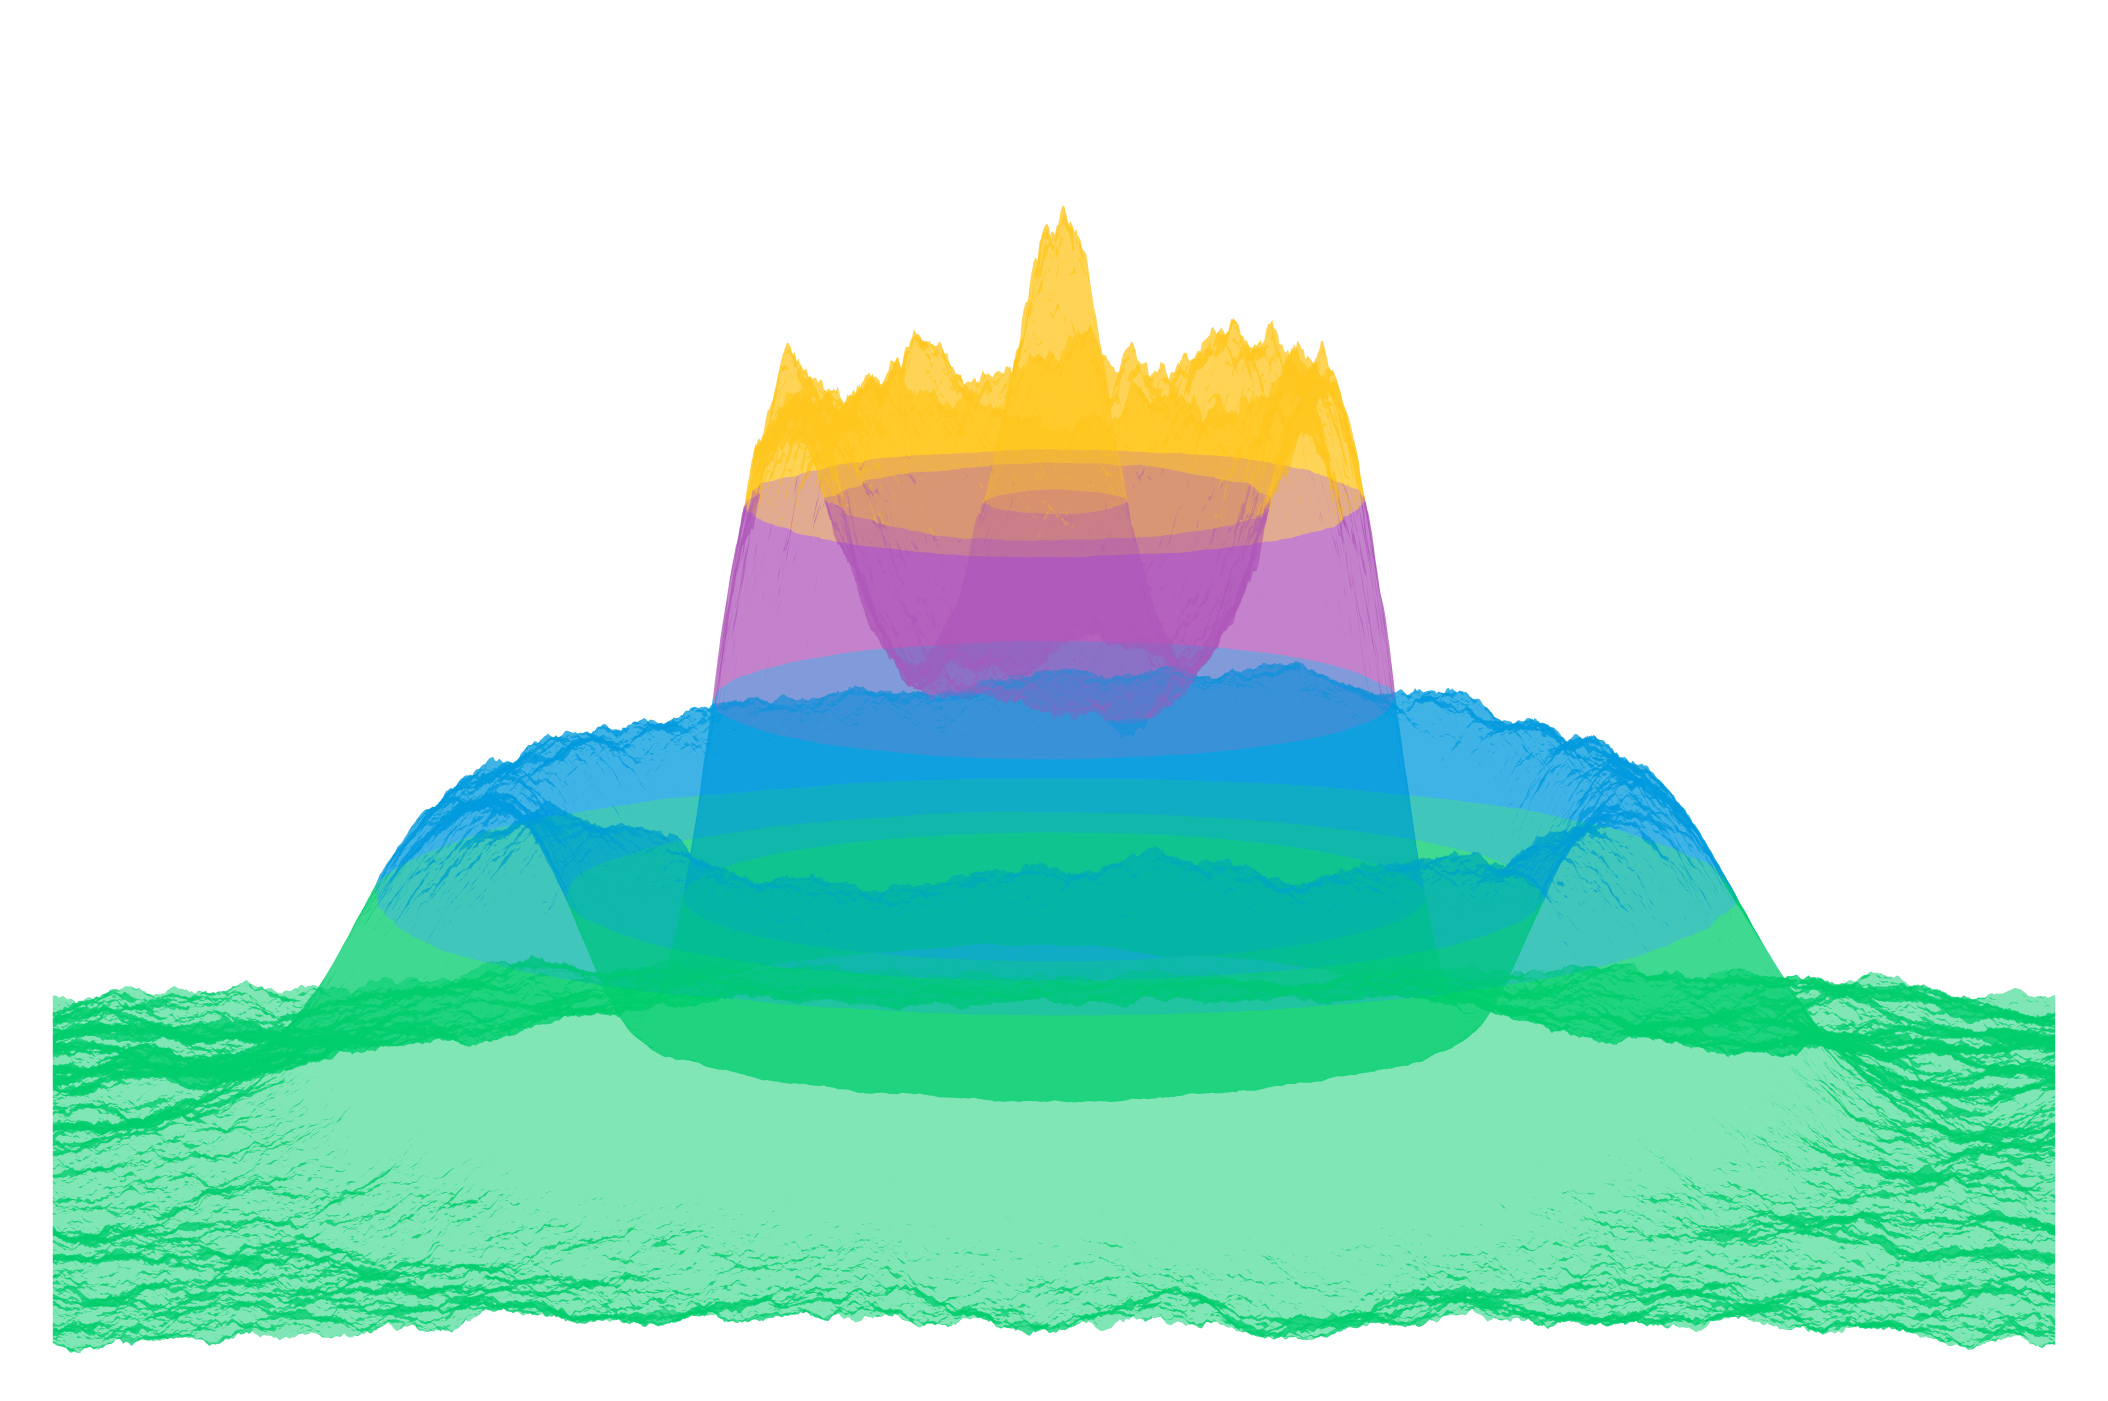
\includegraphics[trim=-350 -800 -700 -300, clip, width=0.4\textwidth]{scripts/figures/matching2/full-surf_side-lowres.png}
  
\includegraphics[trim=0 -800 0 0, width=0.25\textwidth]{scripts/figures/matching2/full-surf_top-lowres.png}
  % \includegraphics[trim=0 0 0 -10, clip, width=\textwidth]{scripts/figures/matching1/817_1024-3_1-1_1.png}
  \caption{The $\hom_1$ persistence diagram of the sinusoidal function pictured to the right.
  Features are colored by birth time, infinite features are drawn above the dotted line.}\label{fig:ripple1}
\end{figure}

Throughout, the four interlevel sets shown correspond to the ranges $[0, 0.3)$, $[0.3, 0.5)$, $[0.5, 0.7)$, and $[0.7, 1)$, respectively.
Our persistent homology computations were done primarily with Dionysus augmented with custom software for computing representative cycles of infinite features.
\footnote{3D figures were made with MayAvi, all other figures were made with Matplotlib.}
The persistent homology of our function was computed with the lower-star filtration of the Freudenthal triangulation on an $N\times N$ grid over $[-1,1]\times[-1,1]\subset\R^2$.
We take this filtration as $\{\rips^{2\delta}(P_\alpha)\}$ where $P$ is the set of grid points and $\delta = \sqrt{2} / N$.

We note that the purpose of these experiments is not to demonstrate the effectiveness of our approximation by Rips complexes, but to demonstrate the relationships between restricted, relative, and truncated diagrams.
Therefore, for simplicity, we will omit the inclusion $\rips^{2\delta}(P_\alpha)\hookrightarrow\rips^{4\delta}(P_\alpha)$ and take the persistent homology of $\{\rips^{2\delta}(P_\alpha)\}$ with sufficiently small $\delta$ as our ground-truth.
% However, in order to keep our diagrams clean we show only those features a distance at least $4\delta$ from the diagonal.
% Note that these features are \emph{not} removed from the diagram, and considered in all computations.

In the following we will take $N = 1024$, so $\delta\approx 1.4\times 10^{-3}$, as our ground-truth.
Figure~\ref{fig:ripple1} shows the \emph{full diagram} of our function with features colored by birth time.
Therefore, for $\omega = 0.3, 0.5, 0.7$ the \emph{truncated diagram} is obtained by successively removing features in each interlevel set.
Recall the \emph{restricted diagram} is that of the function restricted to the $\omega$ \emph{super}-levelset filtration, and computed with $\{\rips^{2\delta}(P_\alpha\setminus Q_\omega)\}$.
We will compare this restricted diagram with the \emph{relative diagram}, computed as the relative persistent homology of the filtration of pairs $\{\rips^{2\delta}(P_\alpha, Q_\omega)\}$.

\paragraph*{The issue with restricted diagrams.}

% In order to get an initial sense of the difference between relative and restricted diagrams we first compare the bottleneck distance of each to the truncated diagram.
% As we have shown the relative diagram is equal to the truncated diagram with additional infinite features we will remove all infinite features from the bottleneck computation.
% We therefore expect the distance between the relative and truncated diagrams to be zero for $N=1024$.

Figure~\ref{fig:bottleneck} shows the bottleneck distance from the truncated diagram at full resolution ($N = 1024$) to both the relative and restricted diagrams with varying resolution.
Specifically, the function on a $1024\times 1024$ grid is down-sampled to grids ranging from $64\times 64$ to $1024\times 1024$.
We also show the expected bottleneck distance to the true truncated diagram given by the interleaving in Theorem~\ref{thm:interleaving_main_2} in black.

\begin{figure}[htbp]
  \centering
  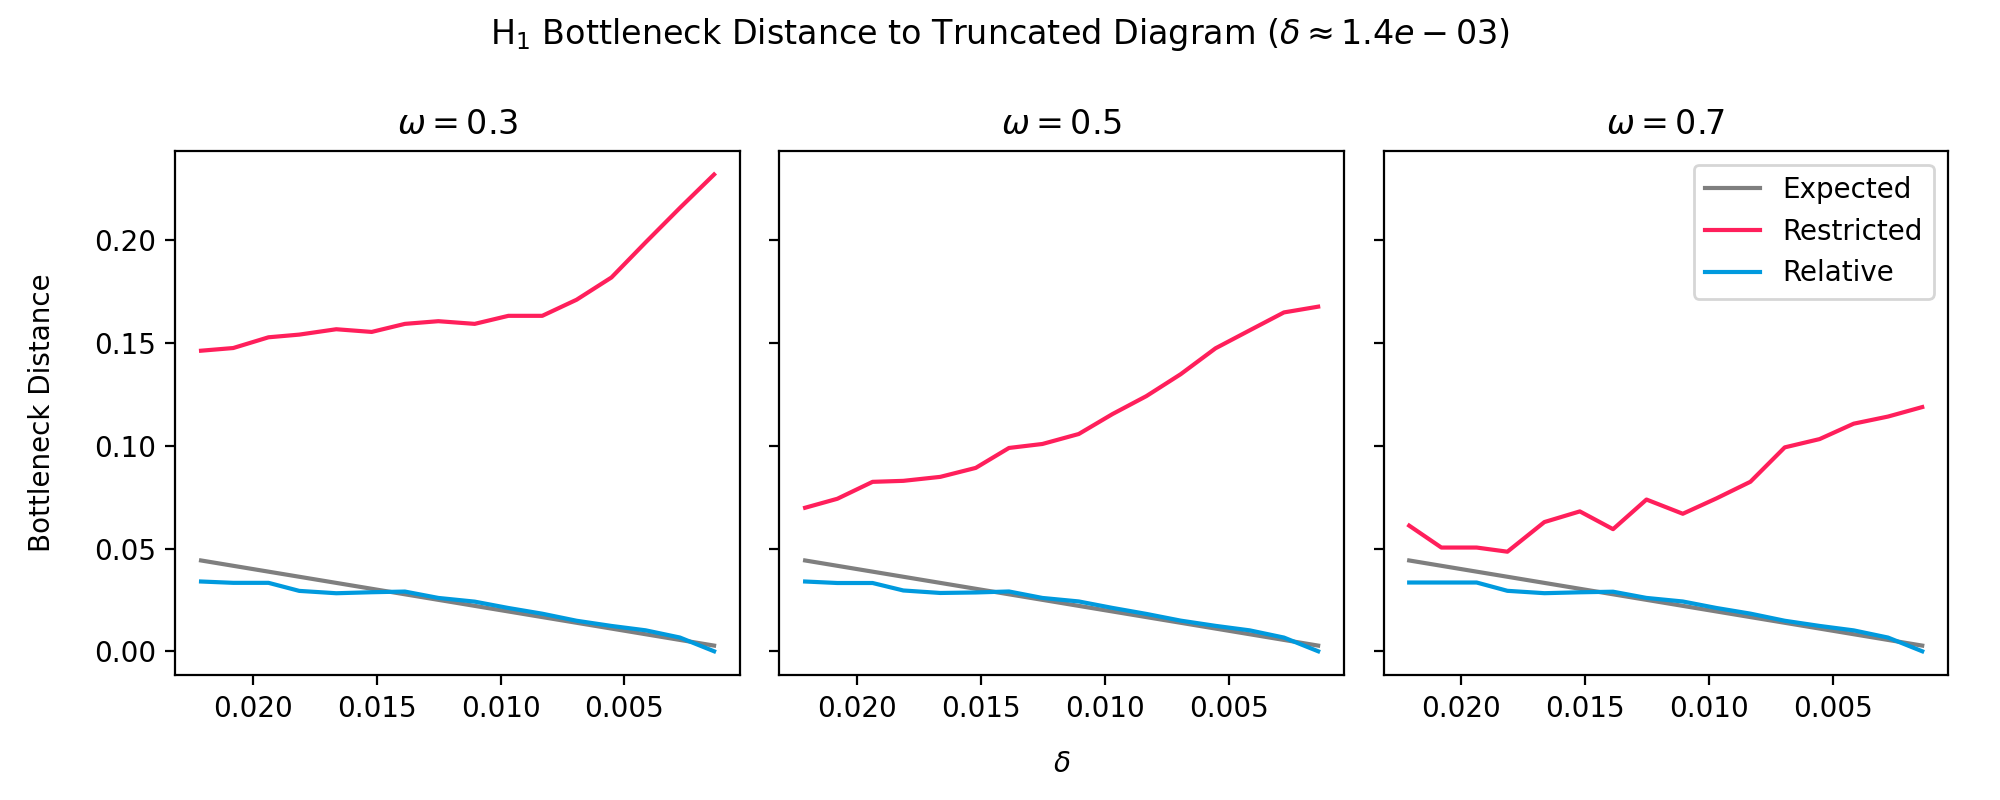
\includegraphics[width=0.95\textwidth]{scripts/figures/matching2/bottleneck_delta.png}
  \caption{Comparison of the bottleneck distance between the truncated diagram and those of the restricted and relative diagrams with increasing resolution.}\label{fig:bottleneck}
\end{figure}

As we can see, the relative diagram clearly performs better than the restricted diagram, which diverges with increasing resolution.
% The reason for this is shown in Figure~\ref{fig:restricted} which depicts the restricted diagrams at $\omega = 0.3, 0.5,$ and $0.7$ at full resolution.
Recall that 1-dimensional features that are born before $\omega$ and die after $\omega$ become infinite 2-dimensional features in the relative diagram, with birth time equal to the death time of the corresponding feature in the full diagram.
These same features remain 1-dimensional figures in the restricted diagram, but with their birth times shifted to $\omega$.
% Indeed, the resulting restricted diagram may be closer to the full diagram for sufficiently small $\omega$.
% However, the distance will be proportional to the difference between $\omega$ and the true birth time.

\begin{figure}[htbp]
  \centering
  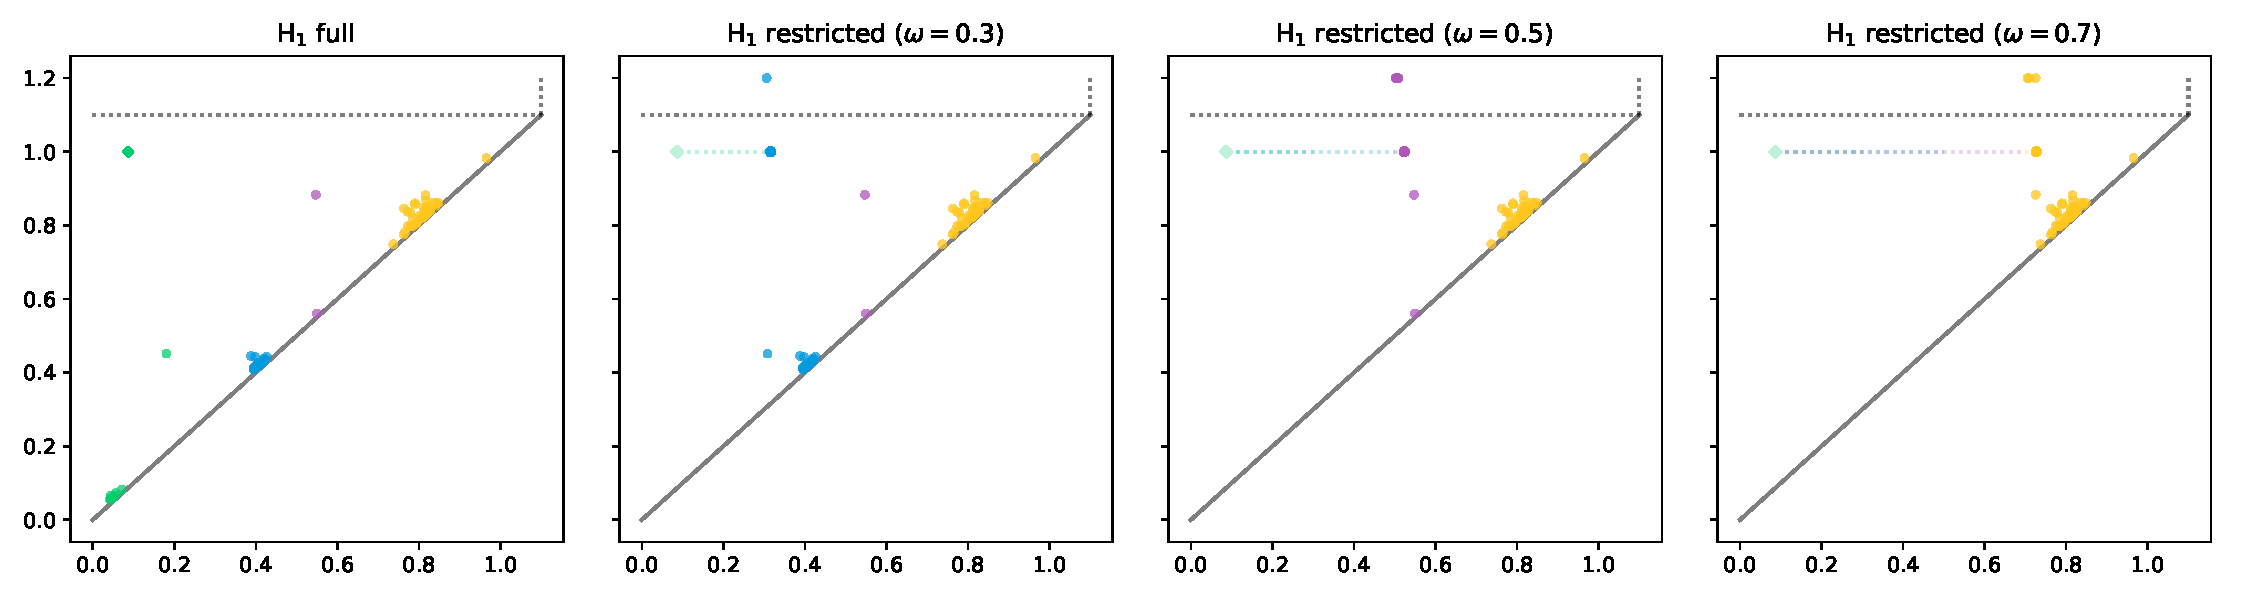
\includegraphics[trim=0 0 -10 0, clip, width=\textwidth]{scripts/figures/matching2/dgm-1.pdf}
  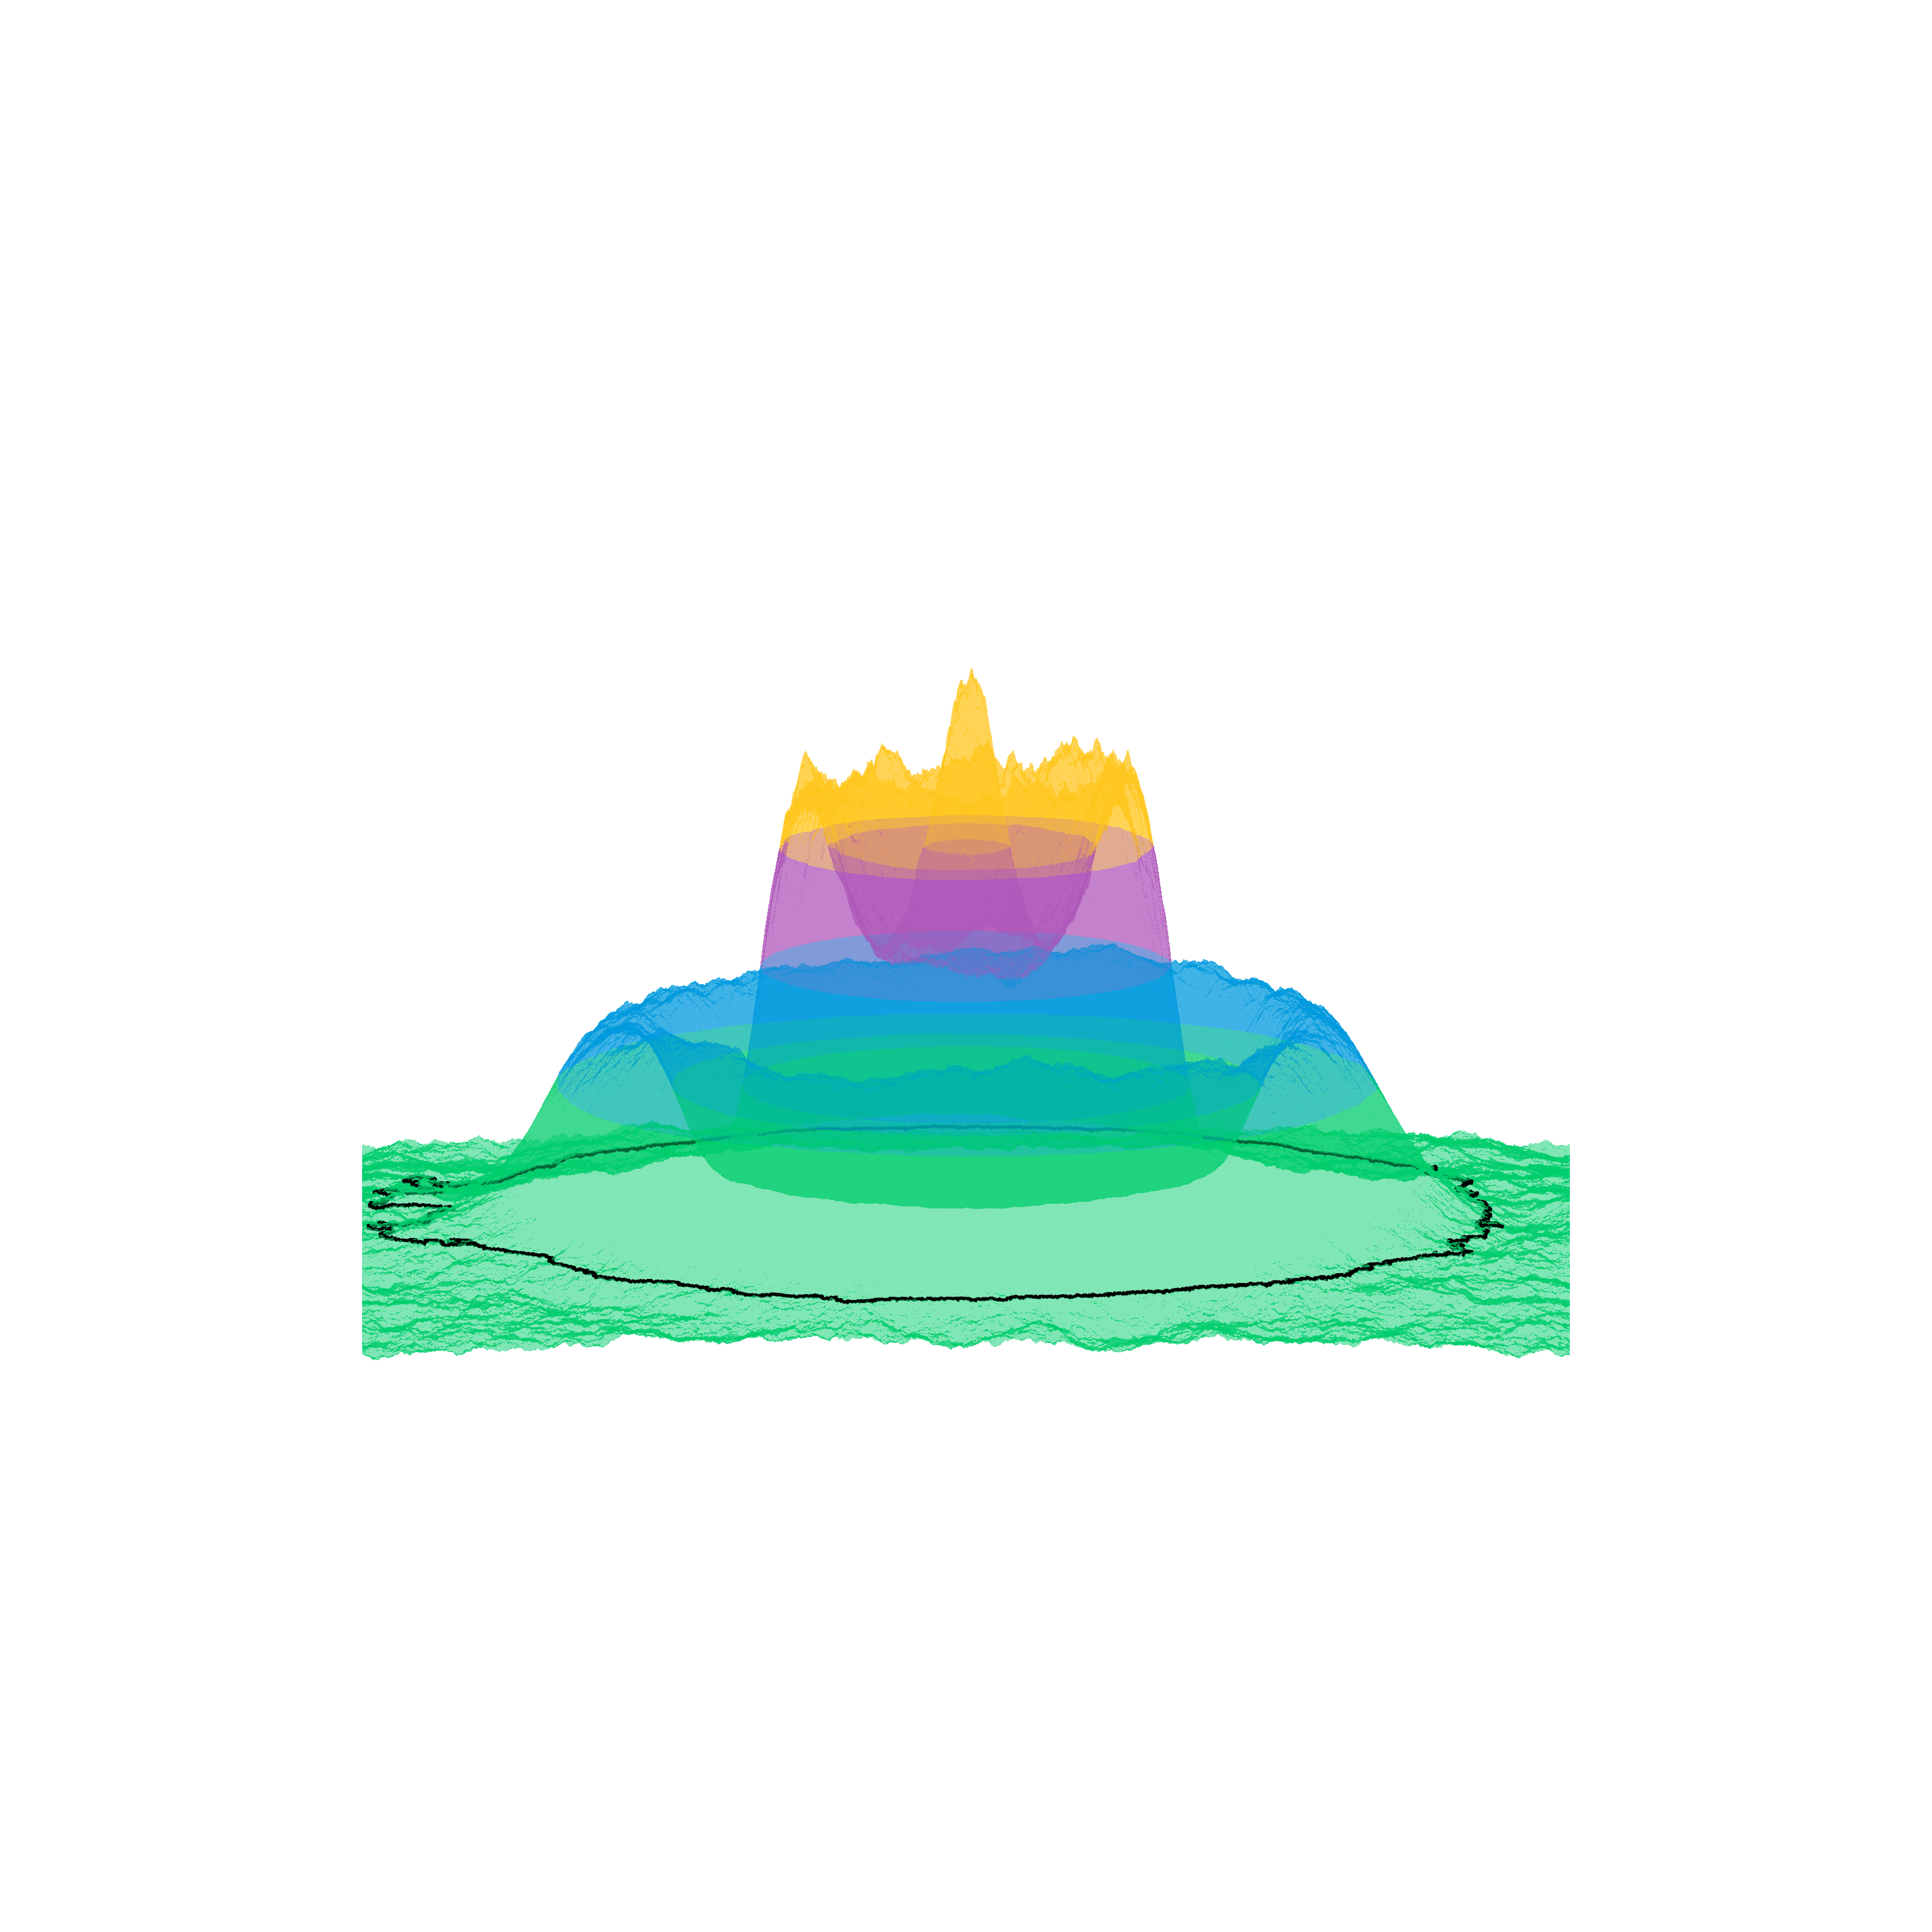
\includegraphics[trim=500 800 500 800, clip, width=0.24\textwidth]{scripts/figures/matching2/surf_side-1.png}
  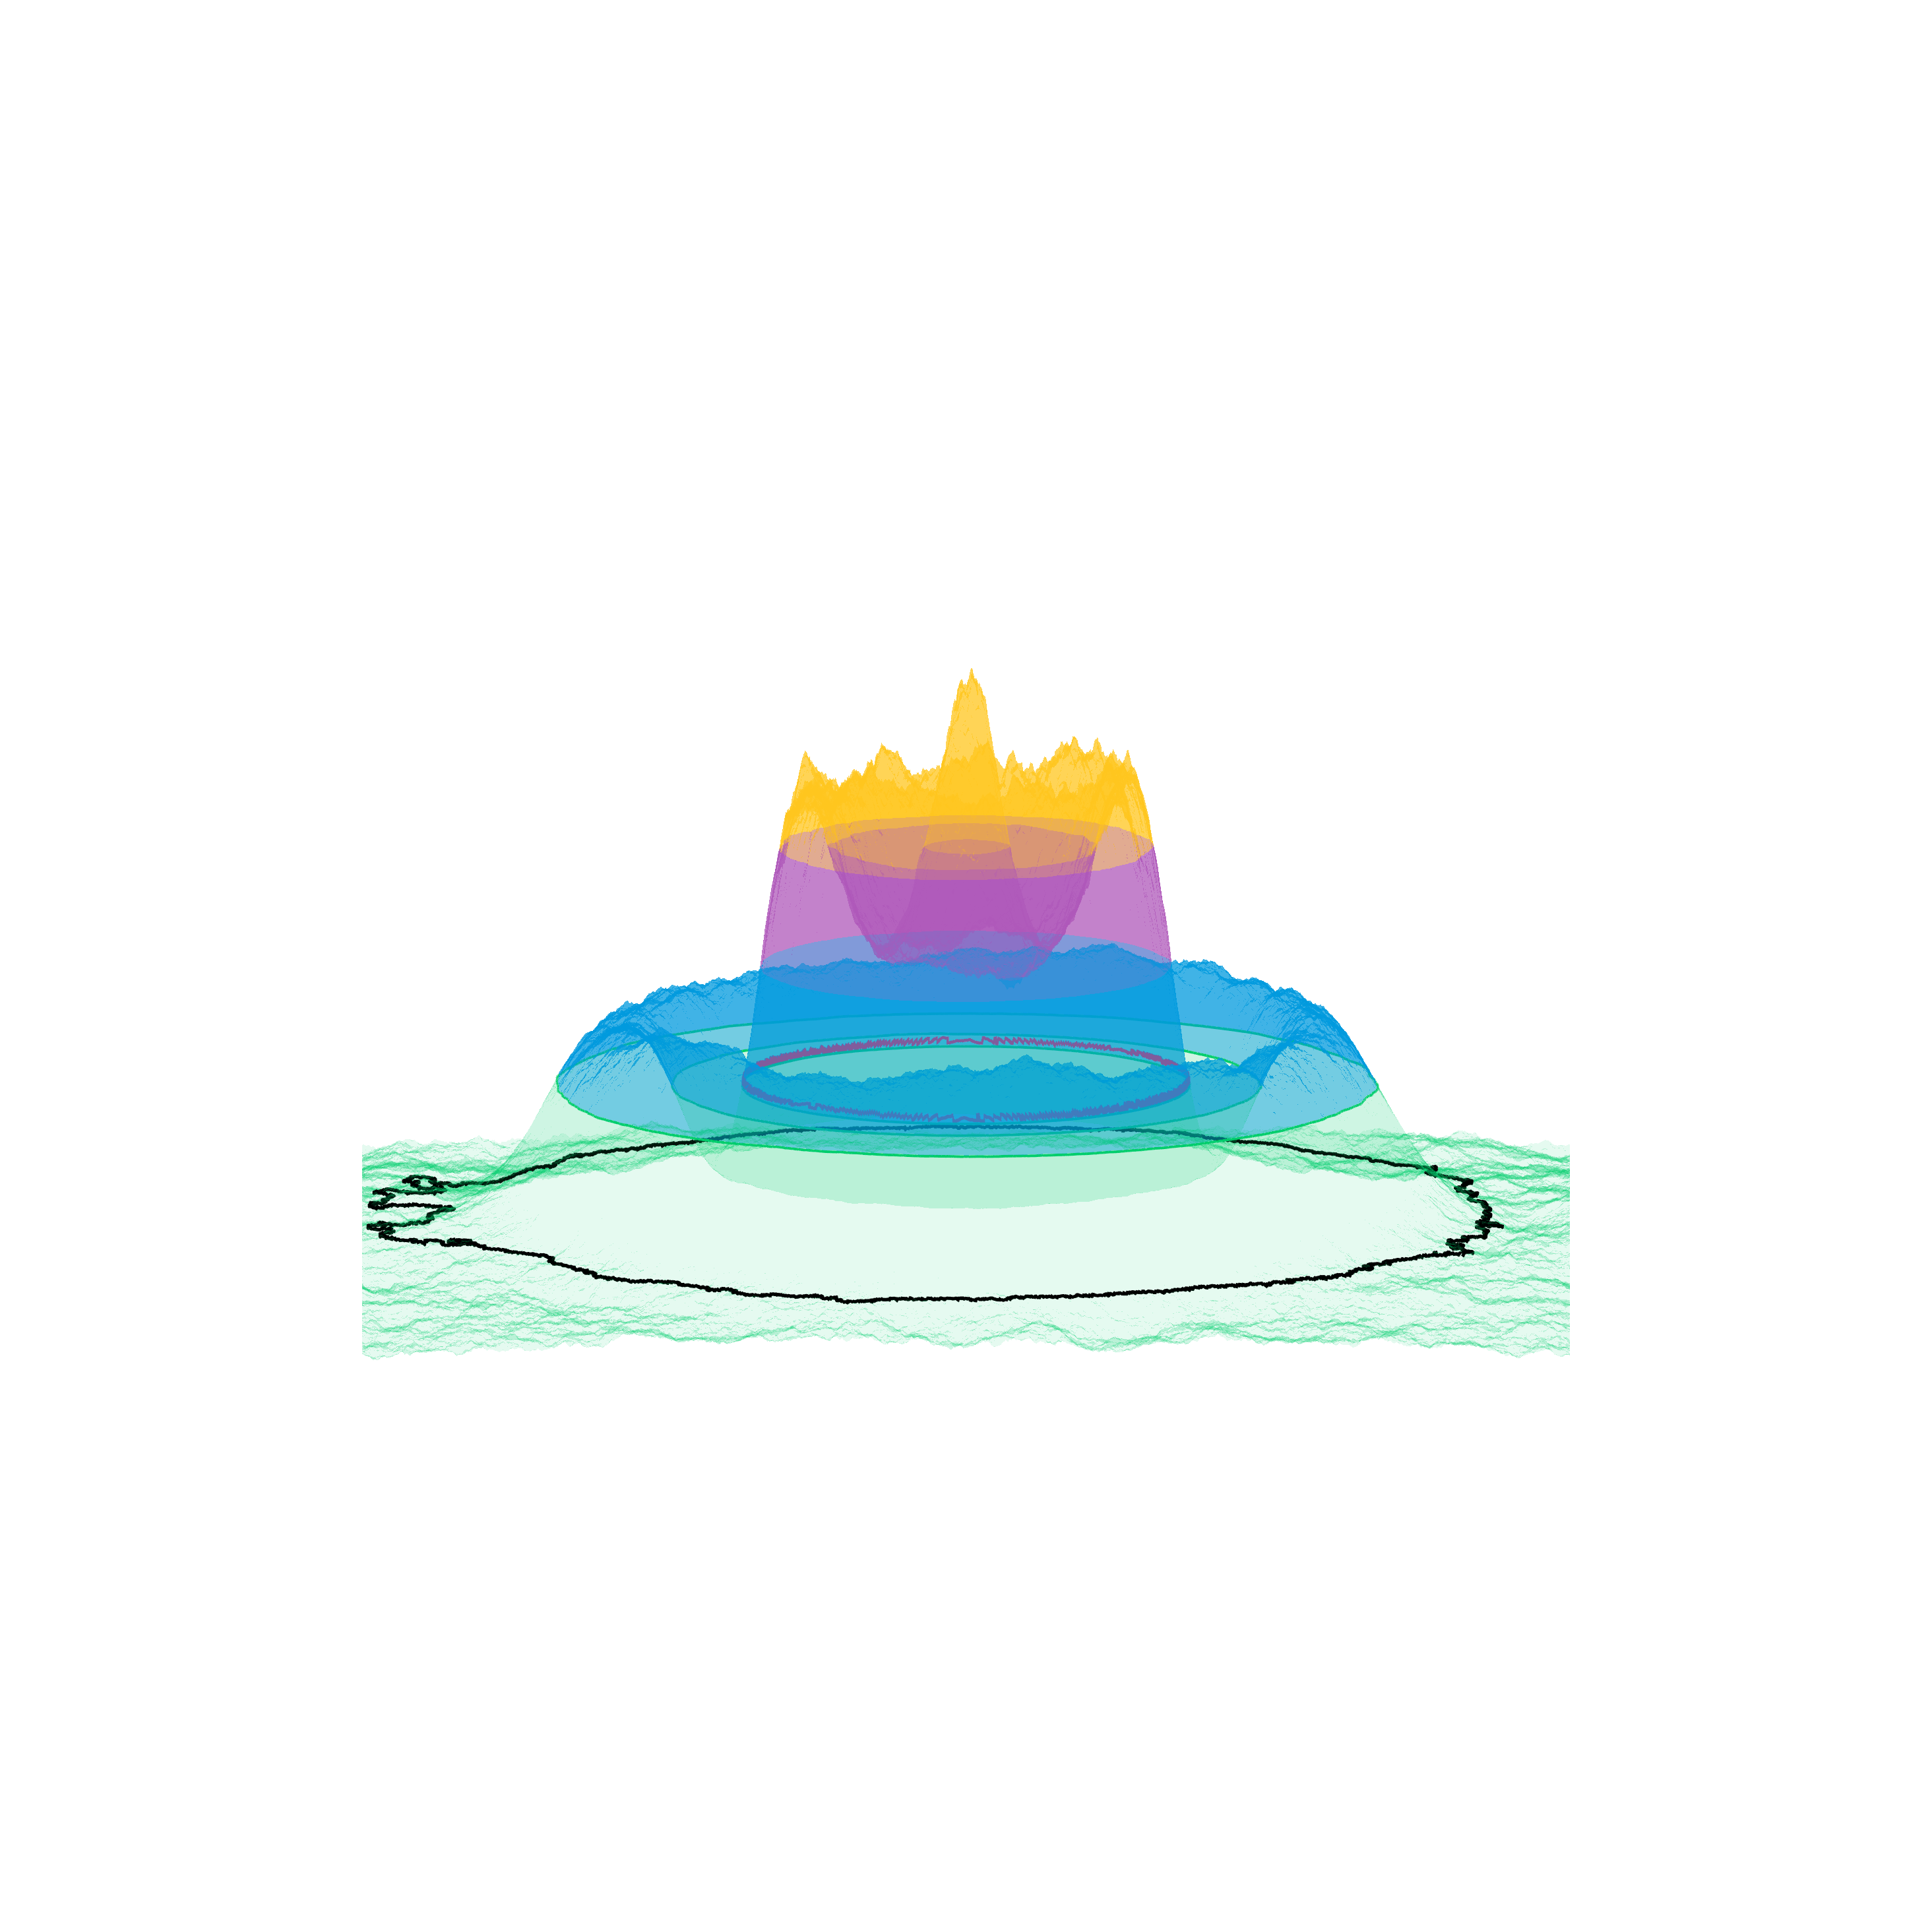
\includegraphics[trim=500 800 500 800, clip, width=0.24\textwidth]{scripts/figures/matching2/surf_side-1_0.png}
  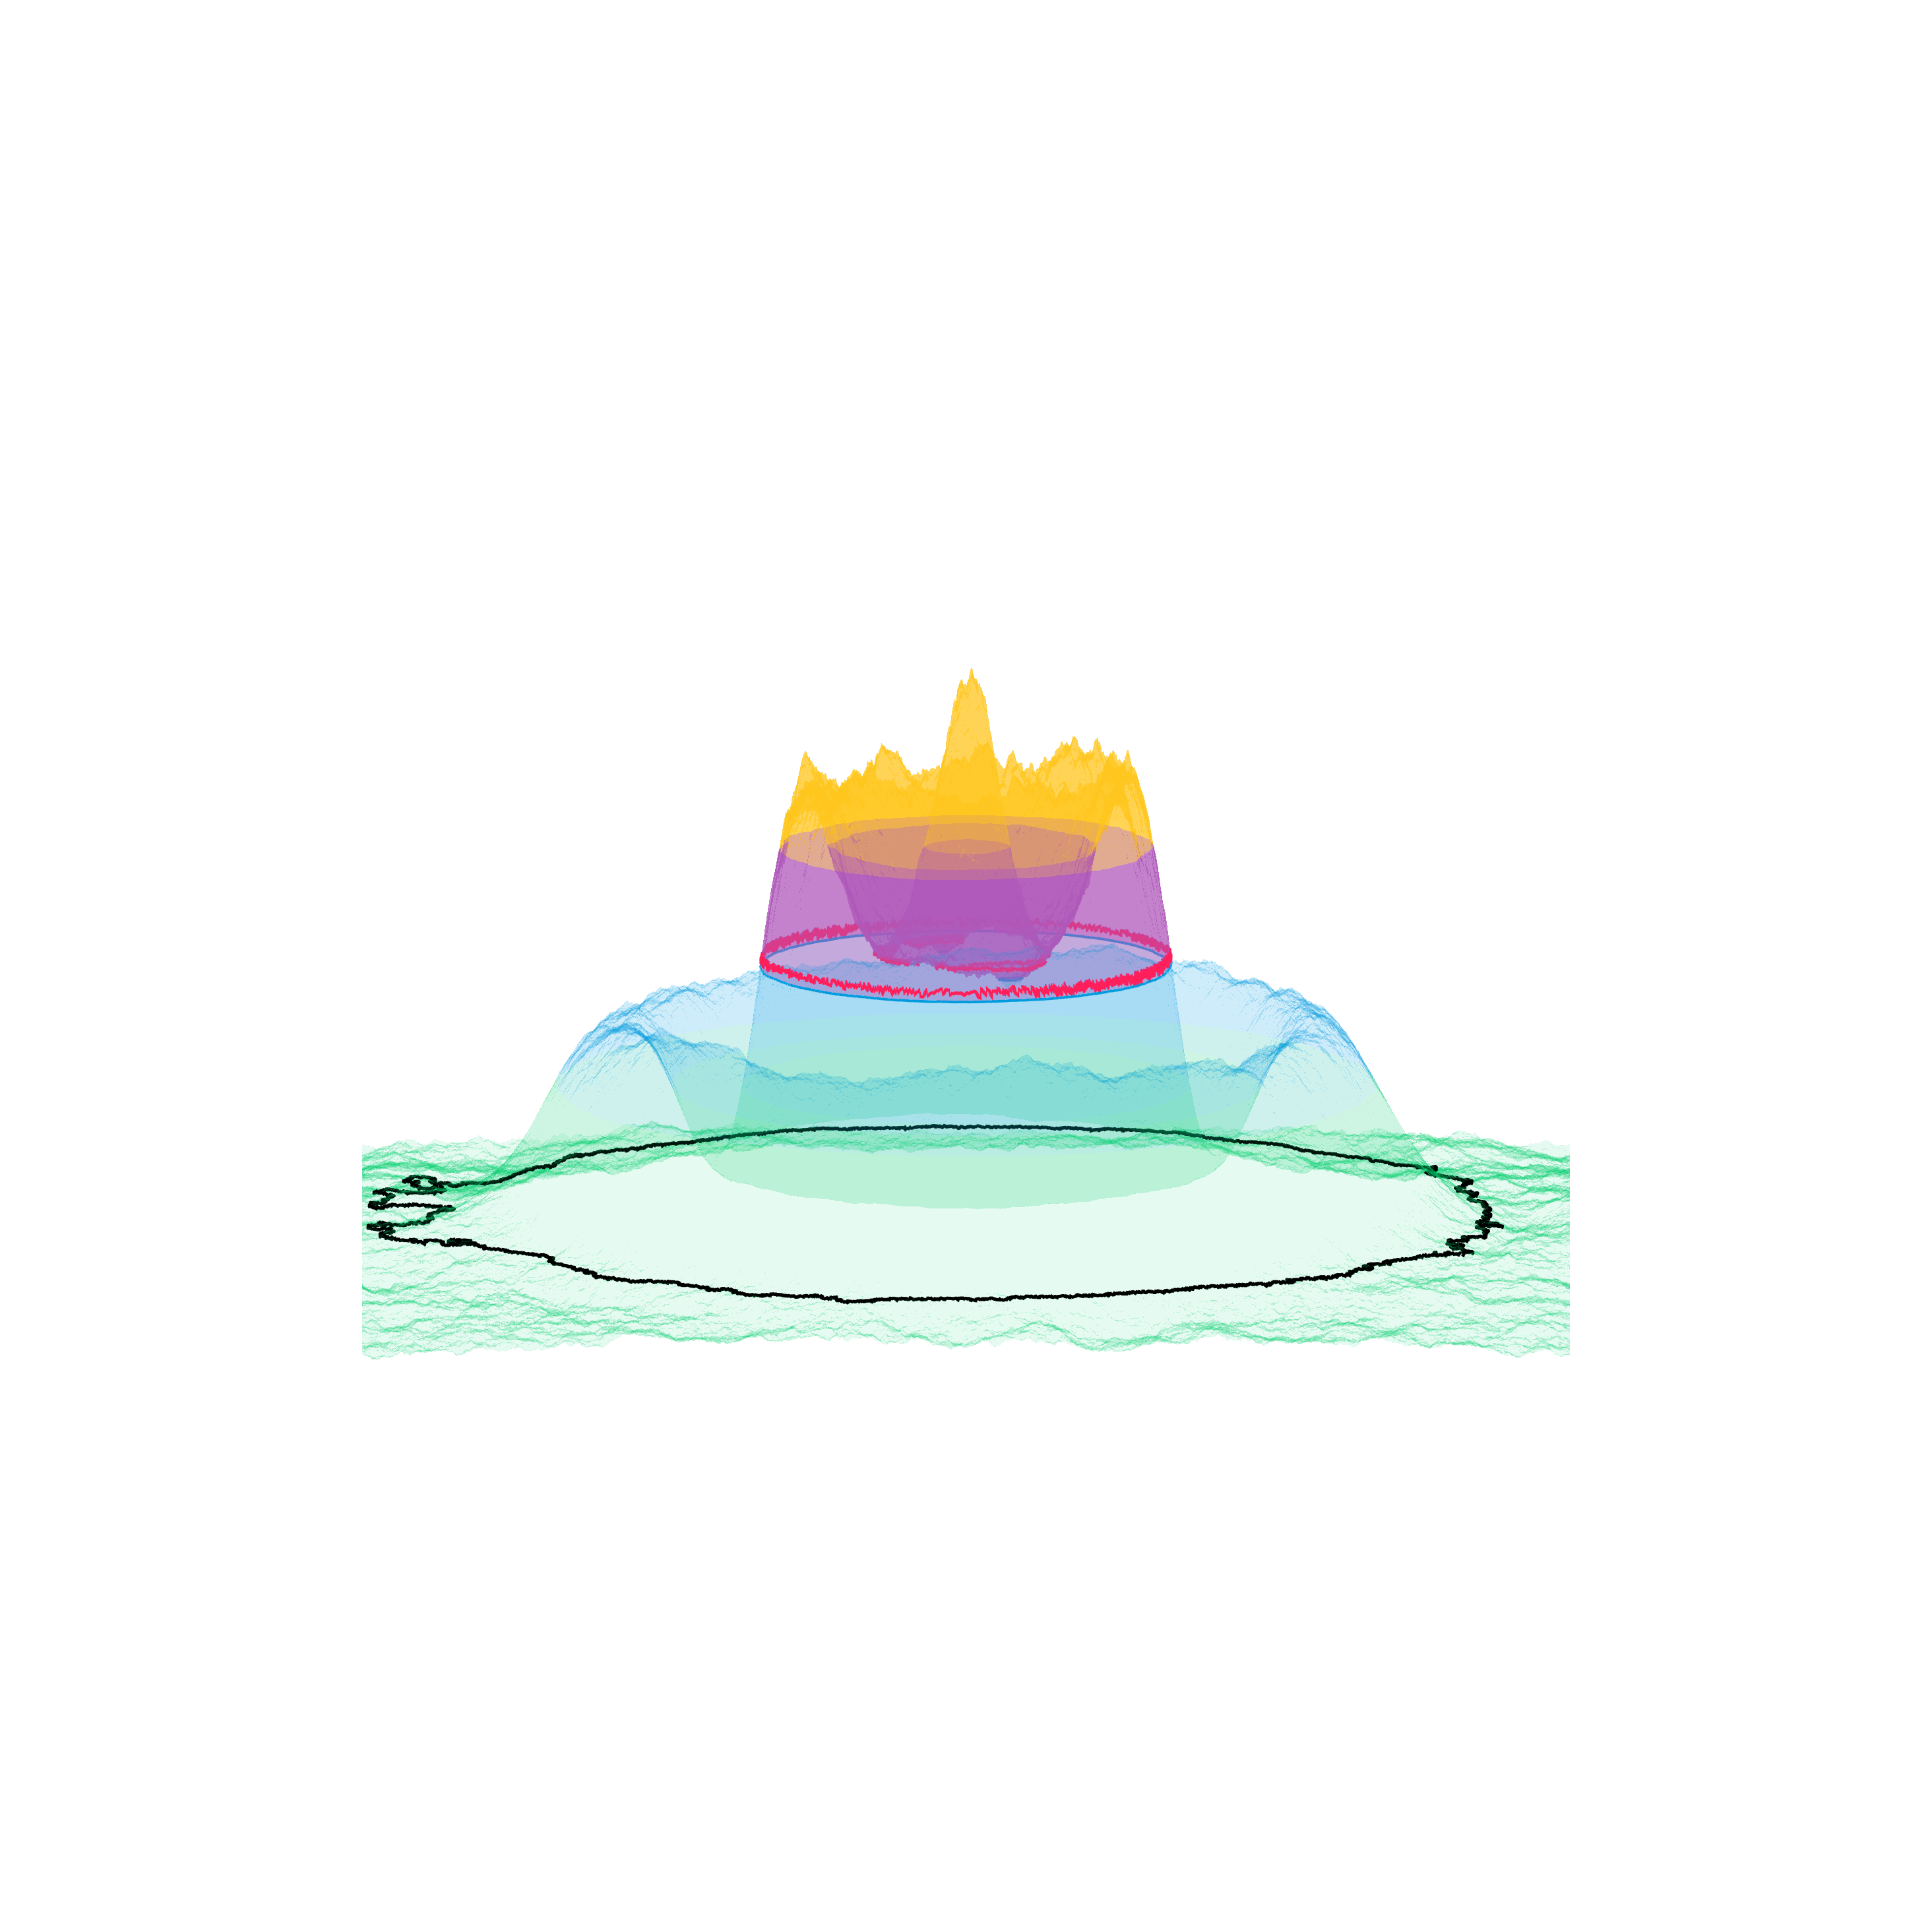
\includegraphics[trim=500 800 500 800, clip, width=0.24\textwidth]{scripts/figures/matching2/surf_side-1_1.png}
  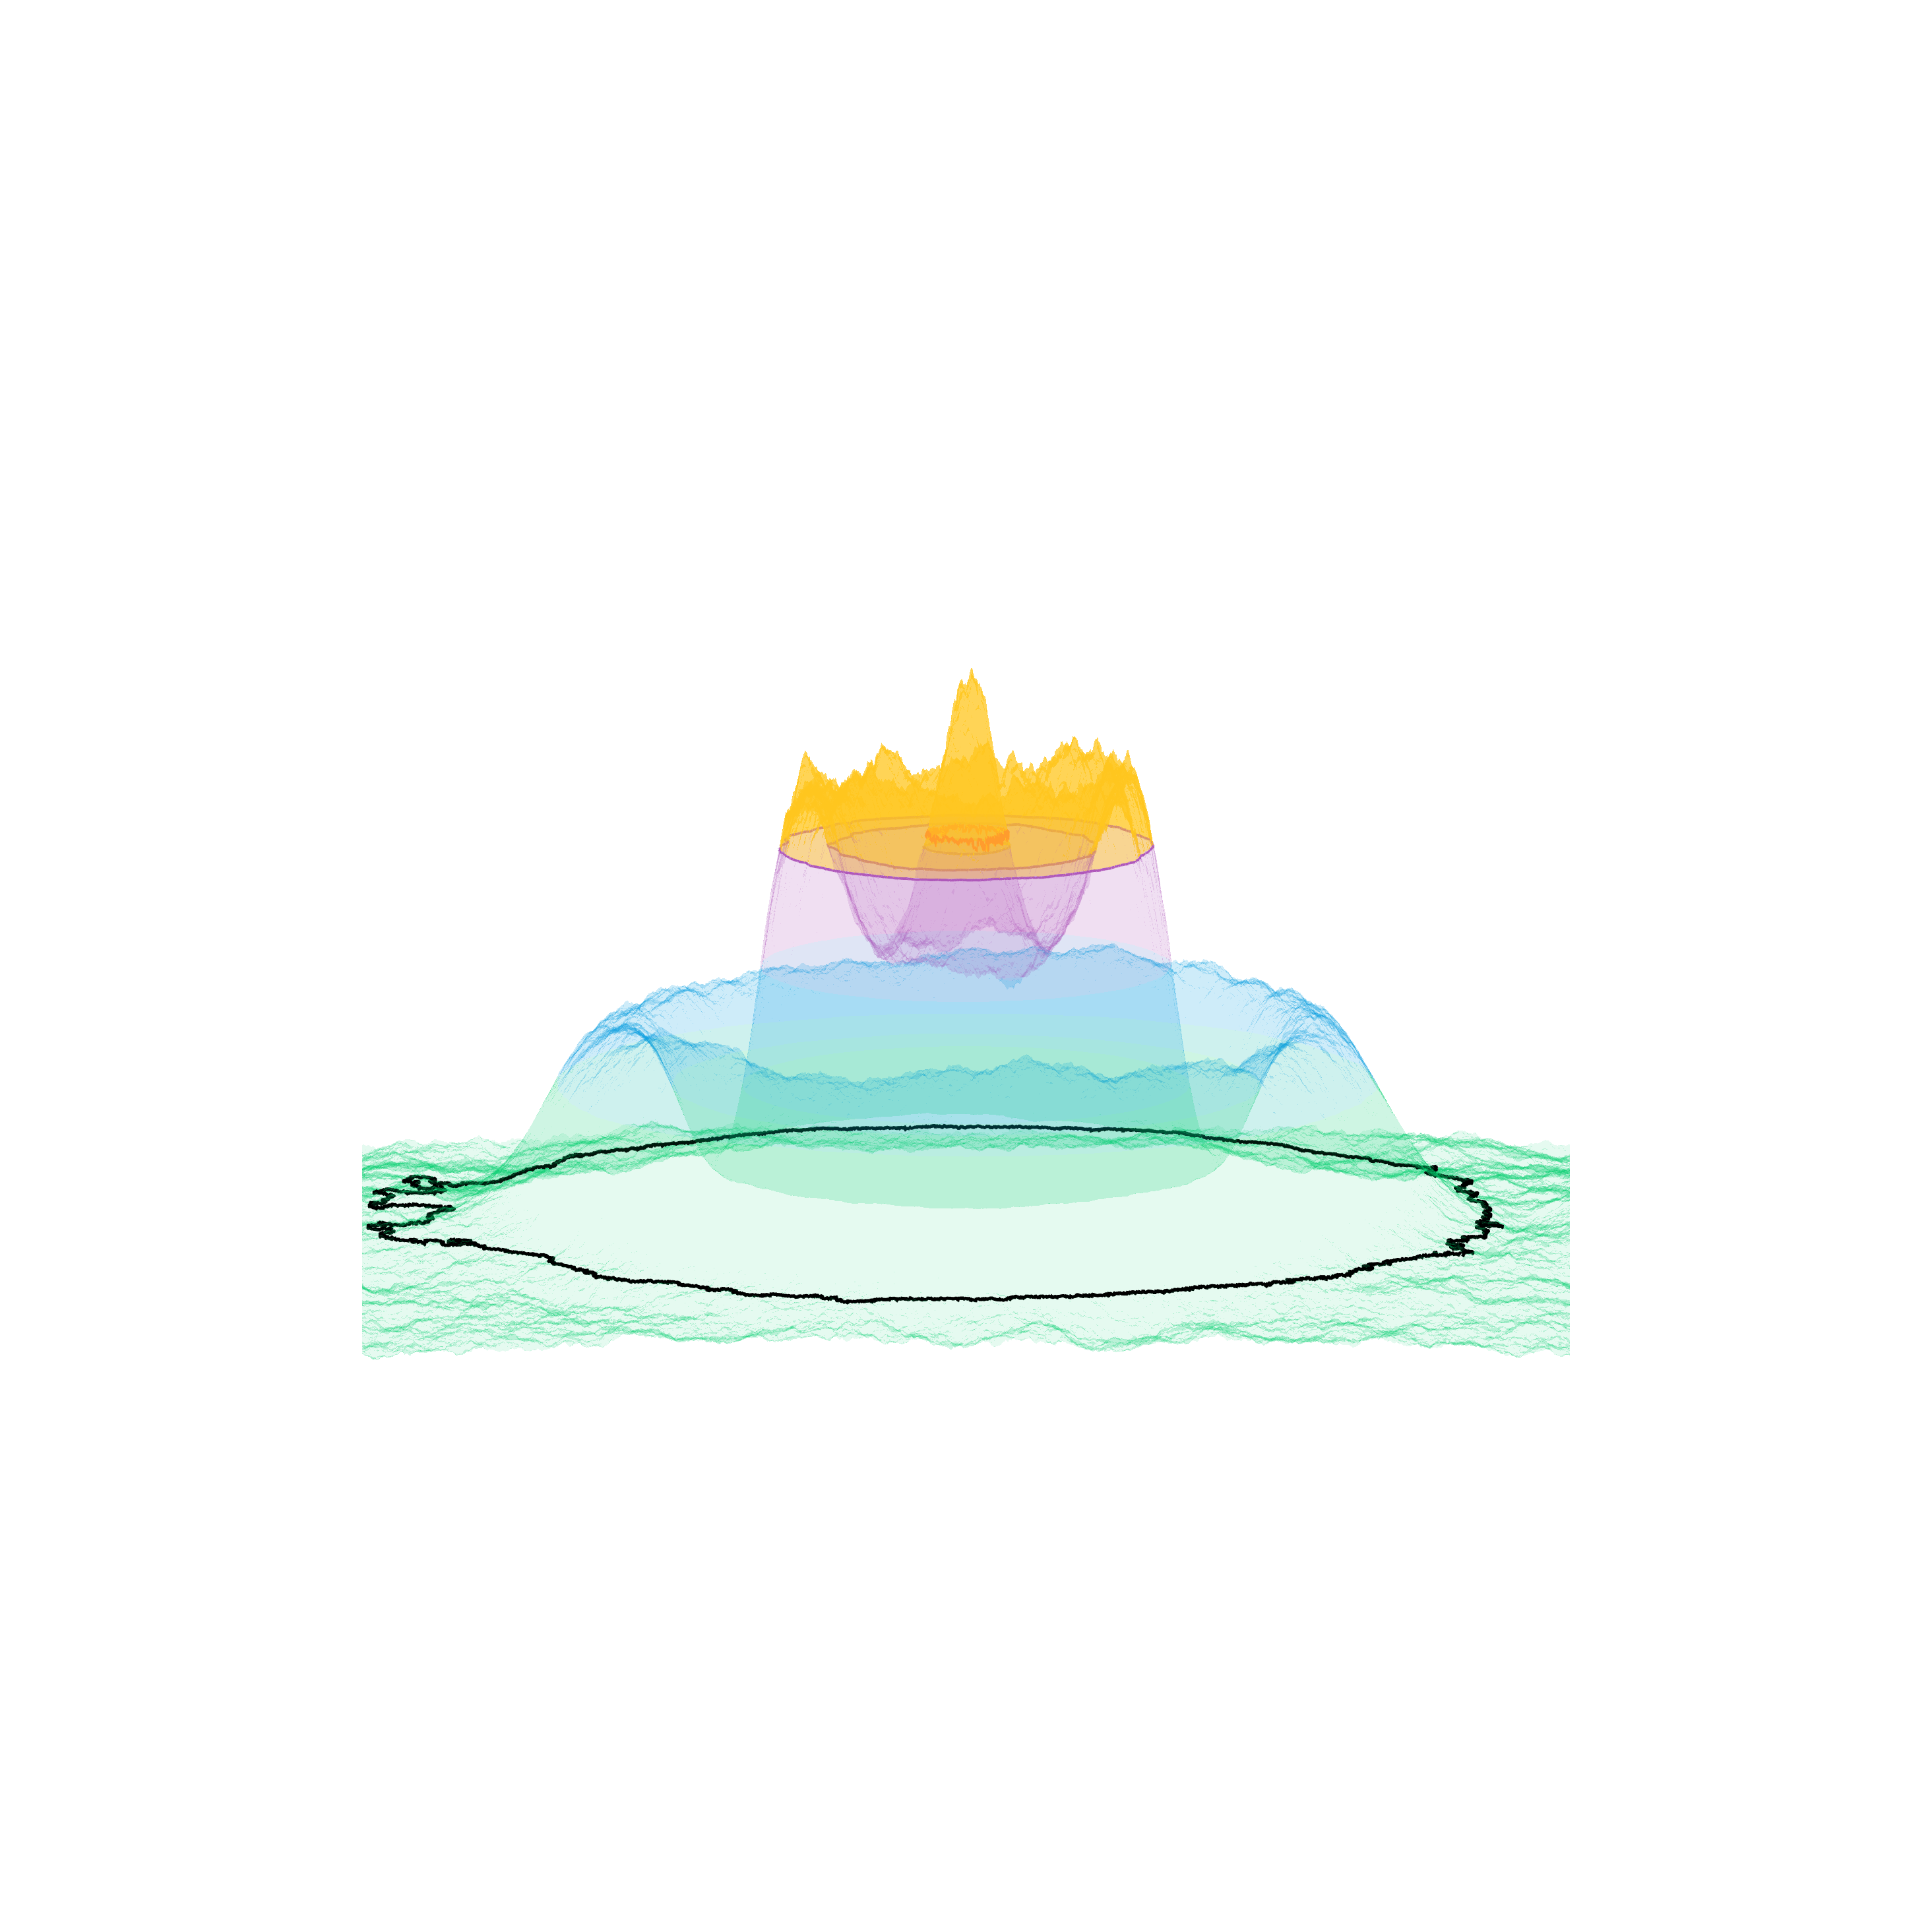
\includegraphics[trim=500 800 500 800, clip, width=0.24\textwidth]{scripts/figures/matching2/surf_side-1_2.png}
  
\includegraphics[trim=500 500 500 500, clip, width=0.24\textwidth]{scripts/figures/matching2/surf_top-1.png}
  
\includegraphics[trim=500 500 500 500, clip, width=0.24\textwidth]{scripts/figures/matching2/surf_top-1_0.png}
  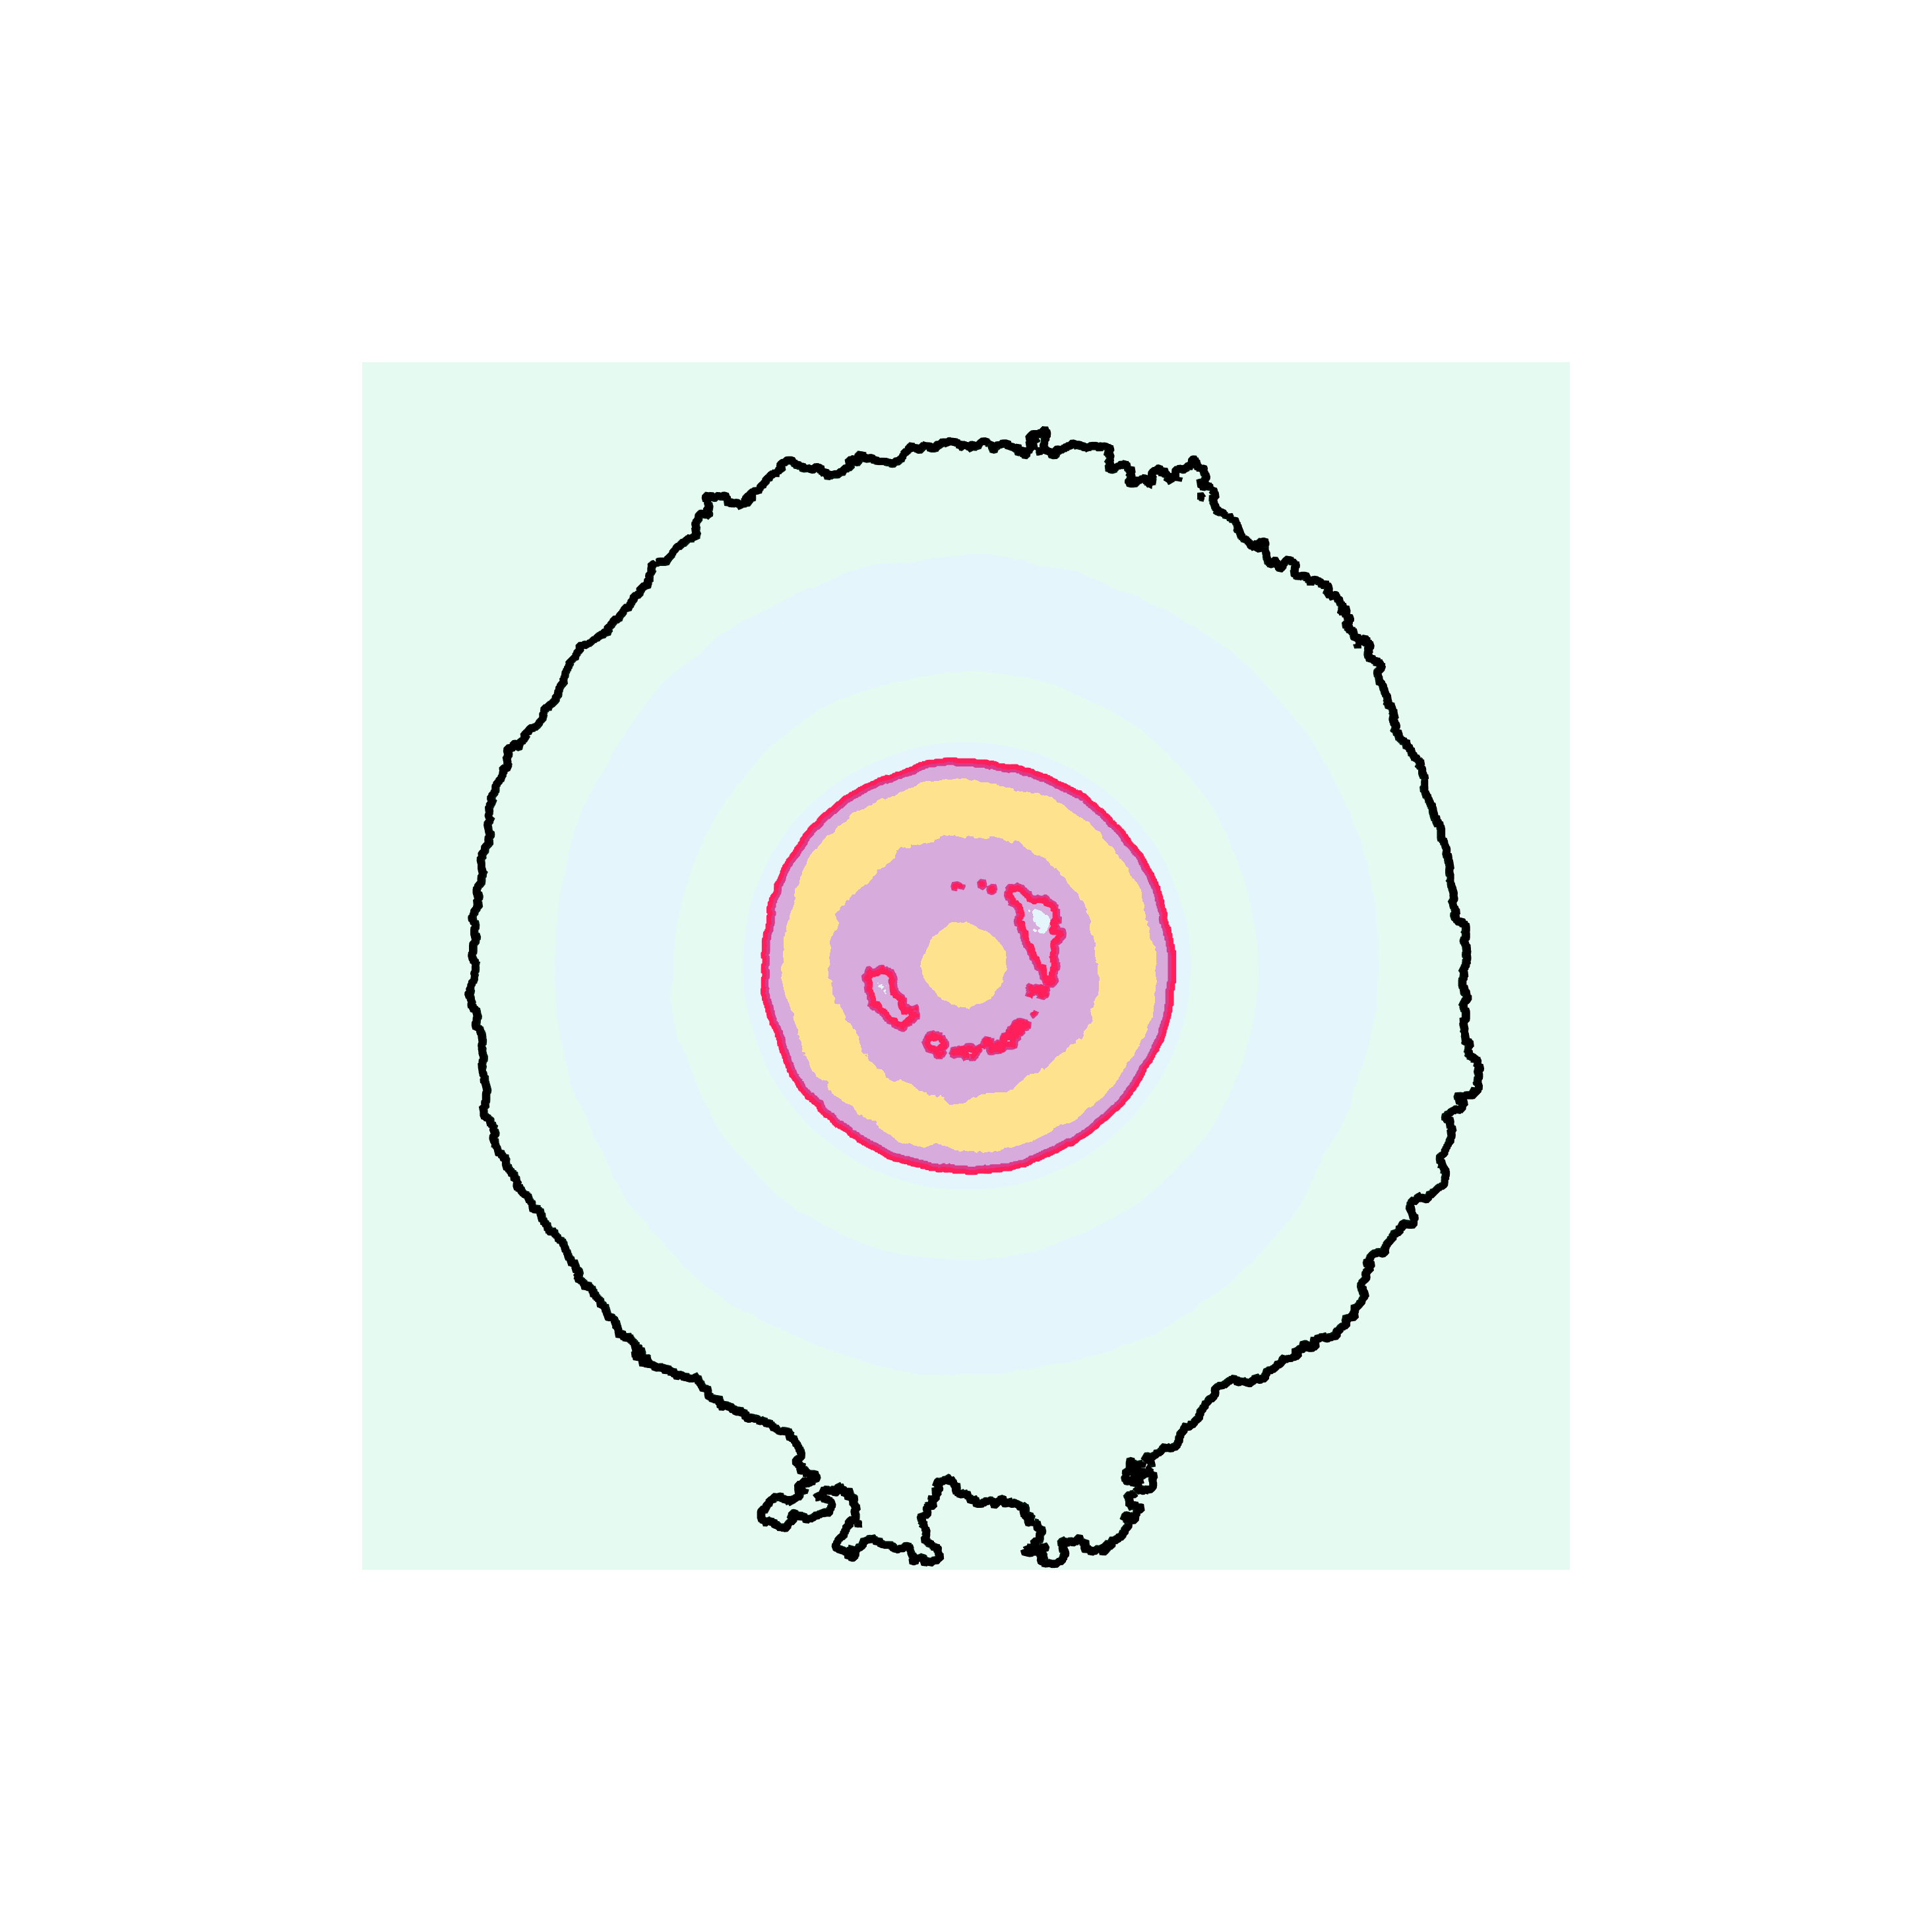
\includegraphics[trim=500 500 500 500, clip, width=0.24\textwidth]{scripts/figures/matching2/surf_top-1_1.png}
  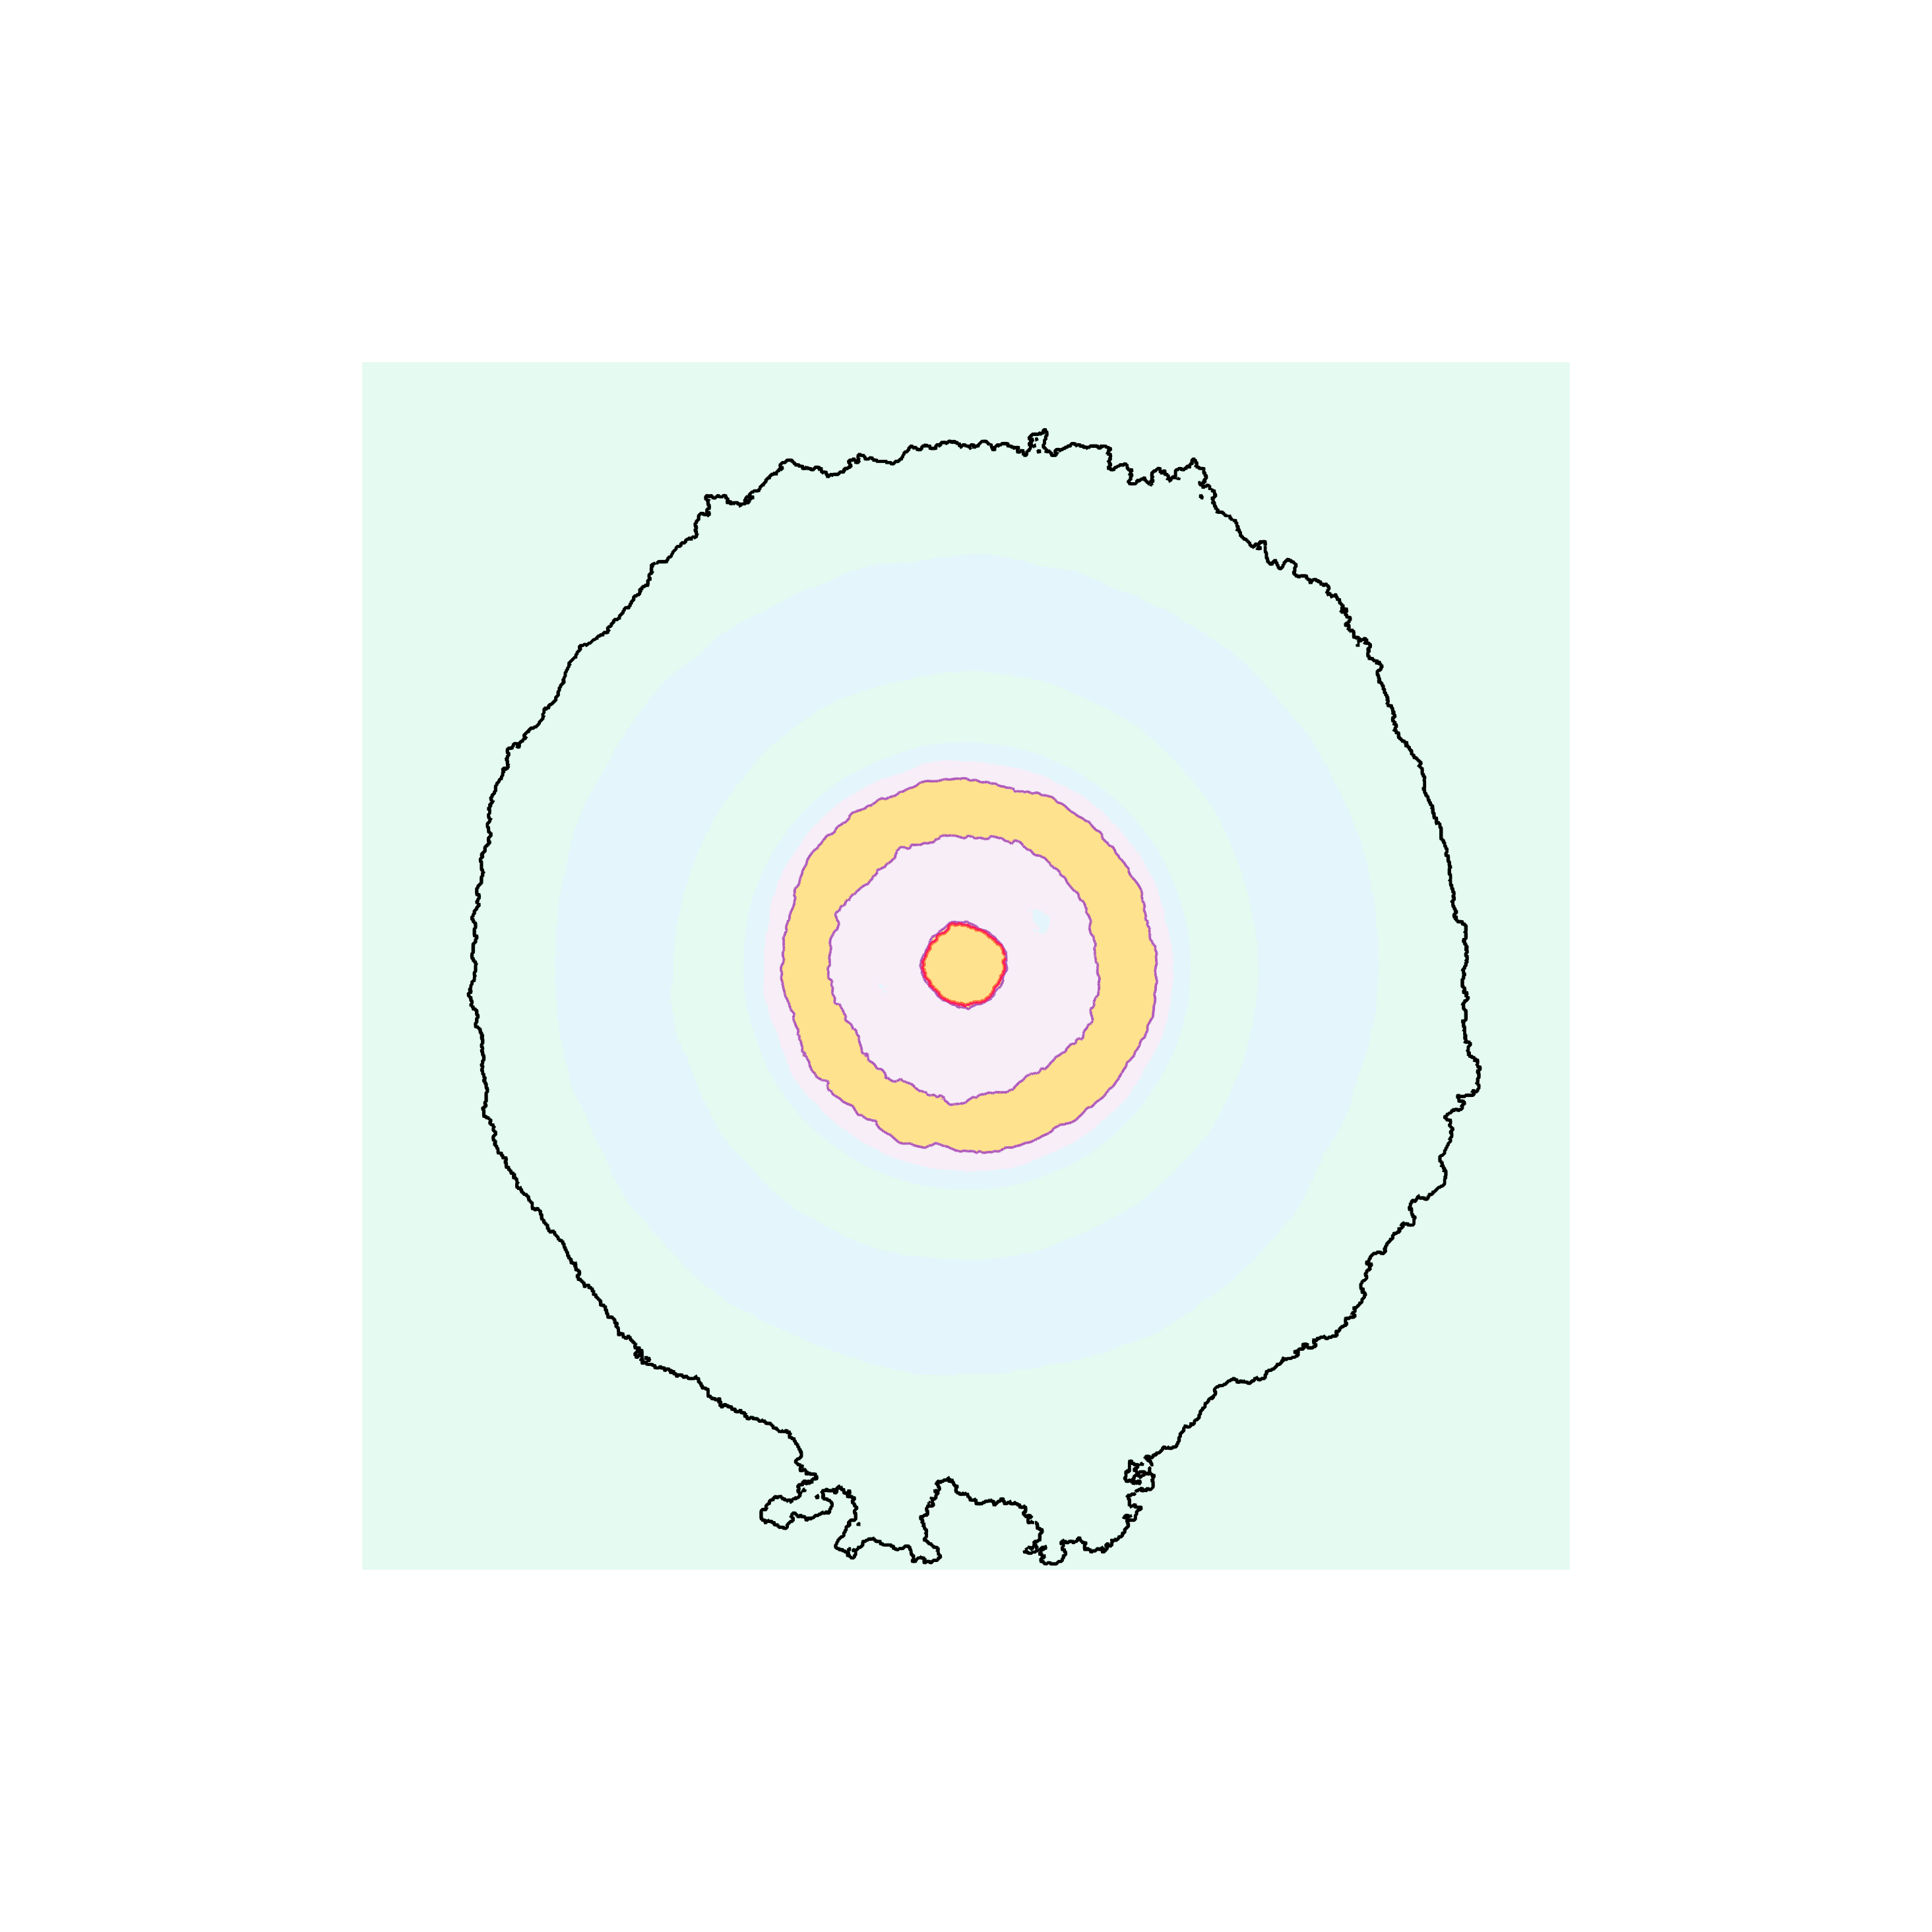
\includegraphics[trim=500 500 500 500, clip, width=0.24\textwidth]{scripts/figures/matching2/surf_top-1_2.png}
  \caption{(Top) $\hom_1$ persistence diagrams of the function depicted in Figure~\ref{fig:ripple1} restricted to \emph{super}-levelsets at $\omega = 0.3, 0.5,$ and $0.7$ (on a $1024\times 1024$ grid).
  The matching is shown between a feature in the full diagram (marked with a diamond) with its representative cycle in black.
  The corresponding representative cycle in the restricted diagram is pictured in red.}\label{fig:restricted}
\end{figure}

Figure~\ref{fig:restricted} shows this distance for a feature that persists throughout the diagram.
As the restricted diagram in full resolution the restricted filtration is a subset of the full filtration, so these features can be matched by their death simplices.
For illustrative purposes we also show the representative cycles associated with these features.

% We imagine a setting where we would like to classify a function using a sample that cannot be verified below some known $\omega$.
% That is, we can only check for coverage of the super-levelset $D\setminus B_\omega$ using the variation of the TCC we have introduced in the previous sections.
% We would then like to classify the function with the bottleneck distance to a set of known functions based on the region we cover.
% However, as we have shown, the restricted diagram may contain artifacts of features born before $\omega$ which will skew our measurement.
% Instead, as $\omega$ is known, we can compare the \emph{relative} diagram the collection of \emph{truncated} diagrams of known functions to get a better classification.

\paragraph*{Relative diagrams and reconstruction.}

\begin{figure}[htbp]
  \centering
  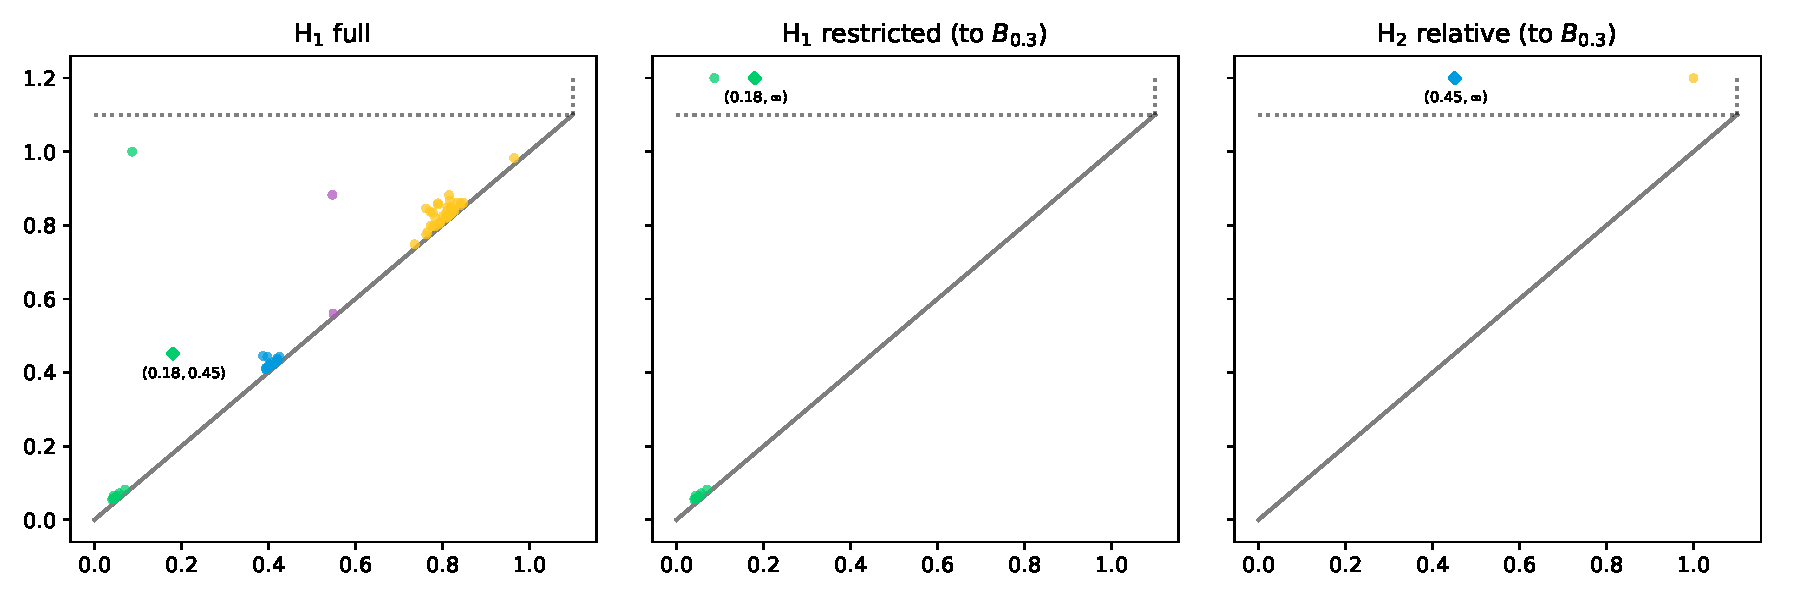
\includegraphics[width=0.9\textwidth]{scripts/figures/relative/dgm-0_0.pdf}
  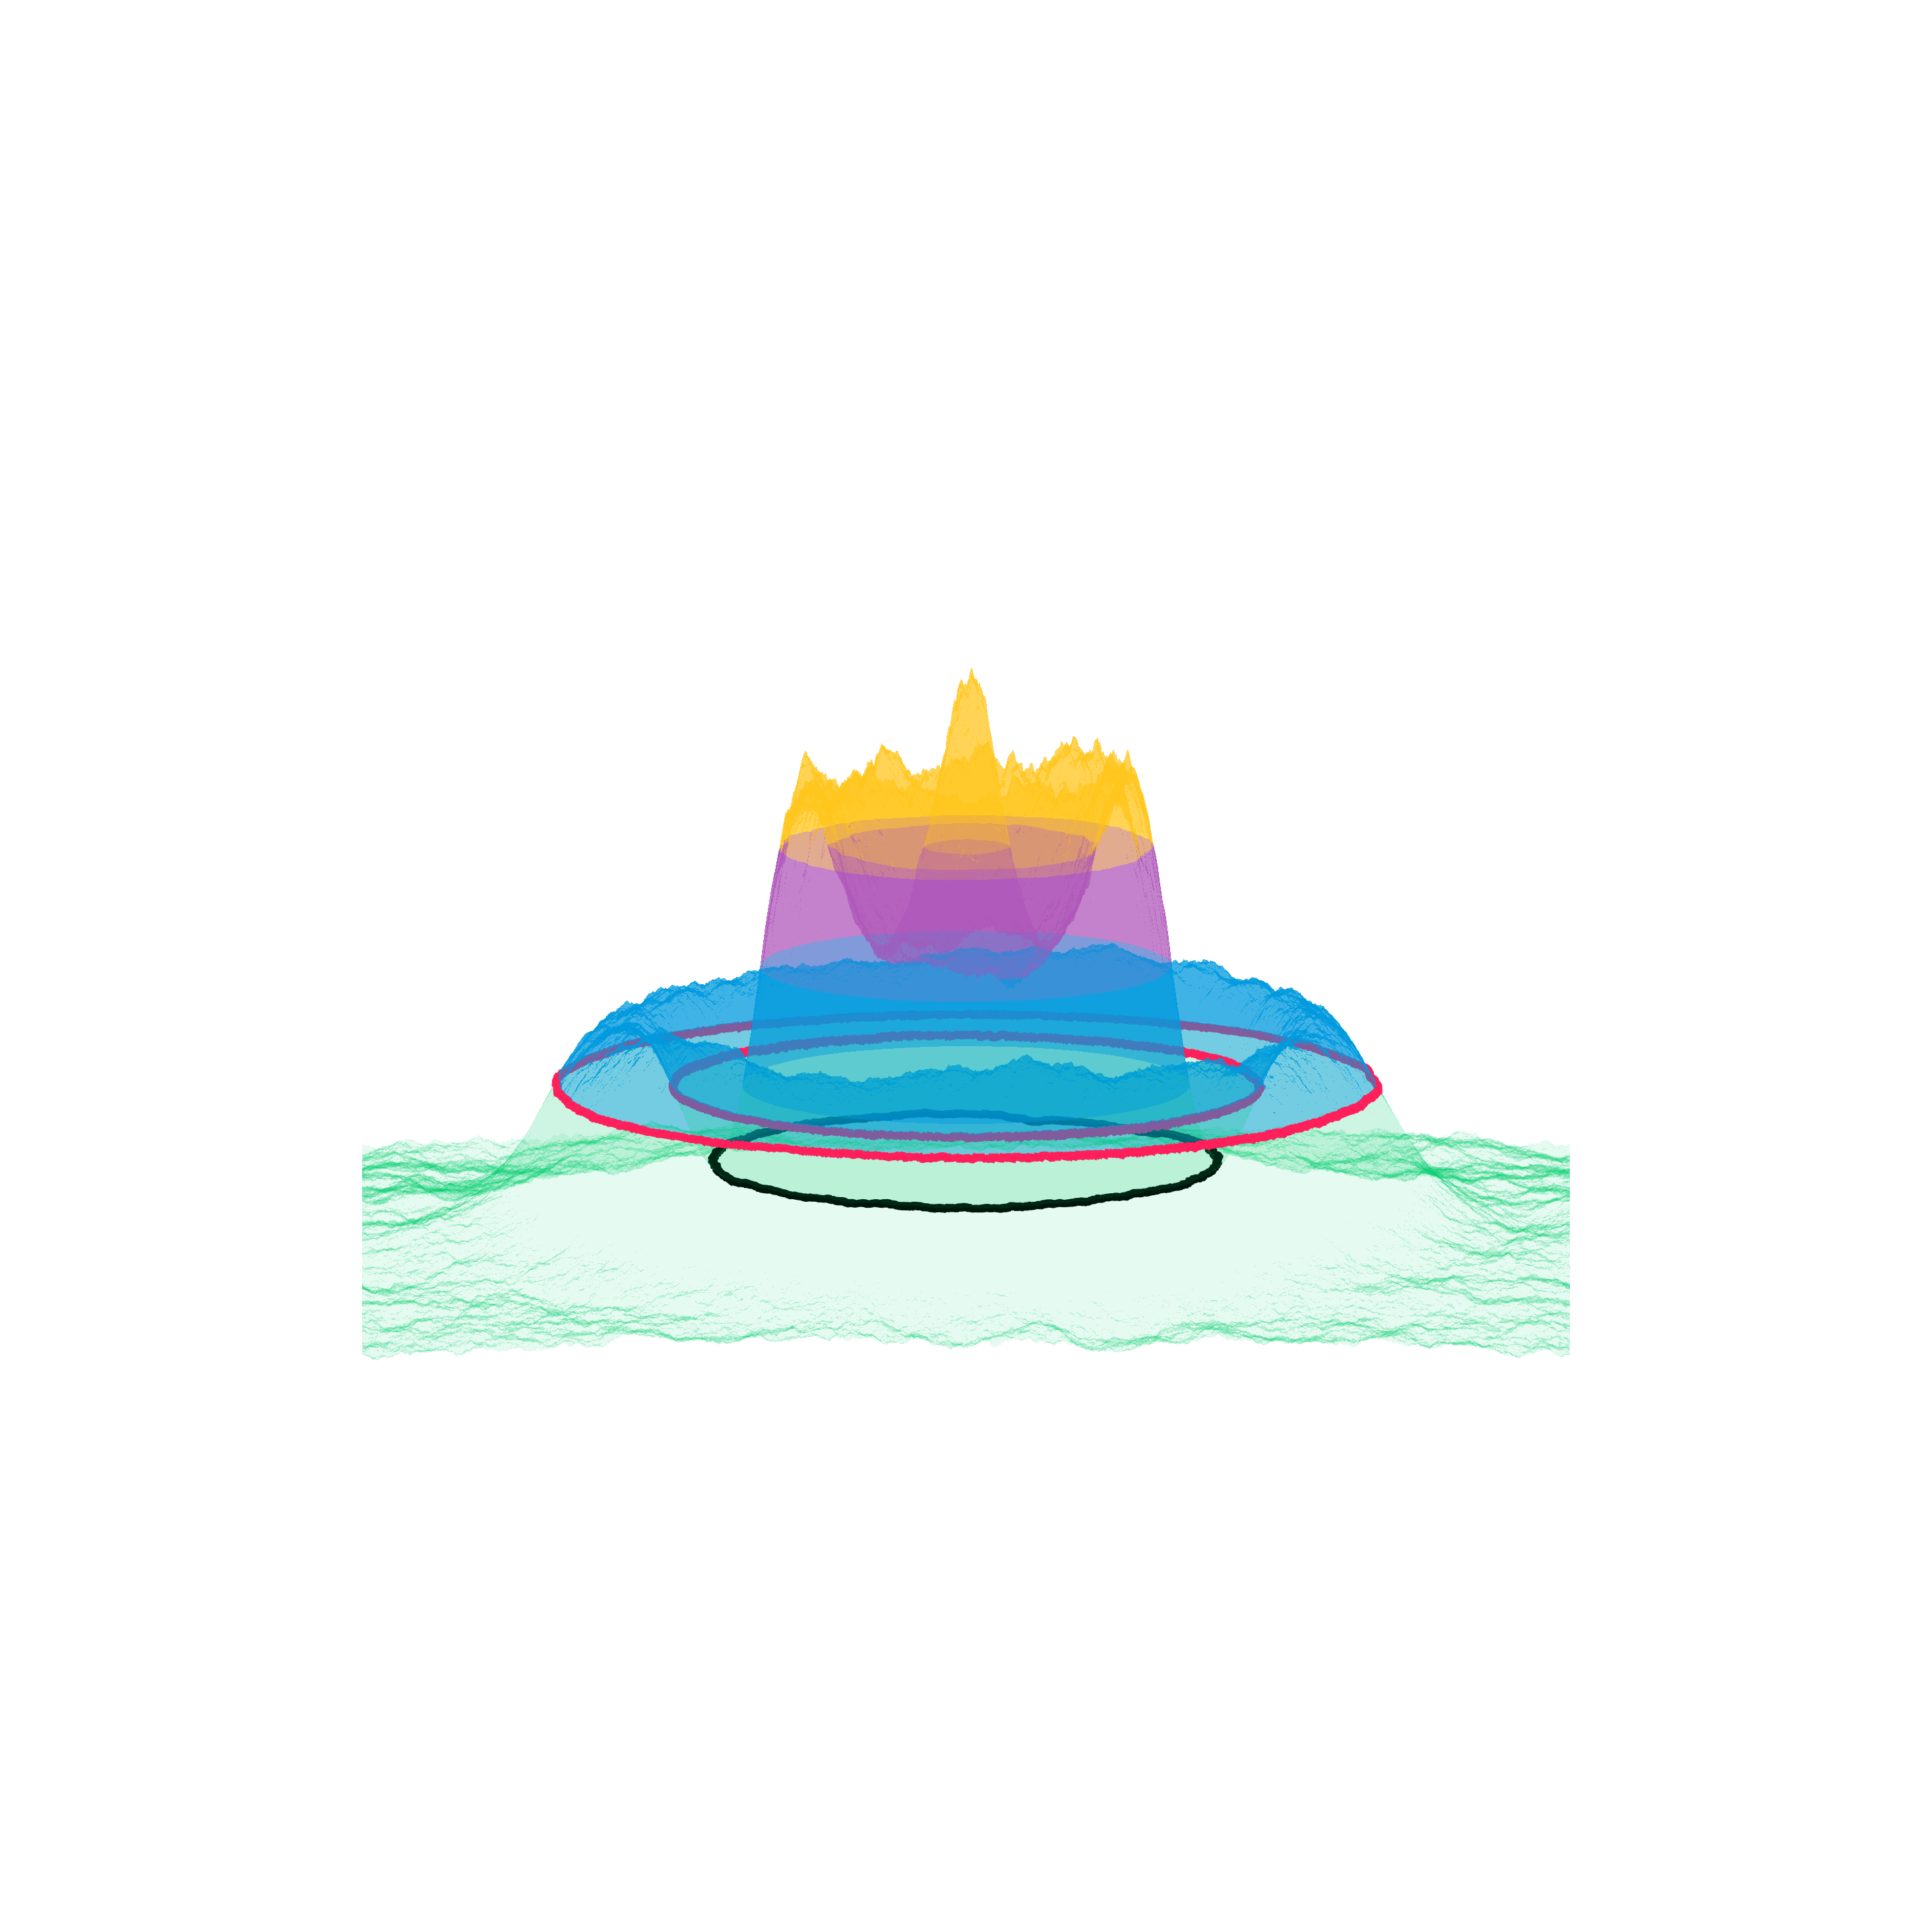
\includegraphics[trim=500 800 500 800, clip, width=0.35\textwidth]{scripts/figures/relative/surf_side-0_0.png}
  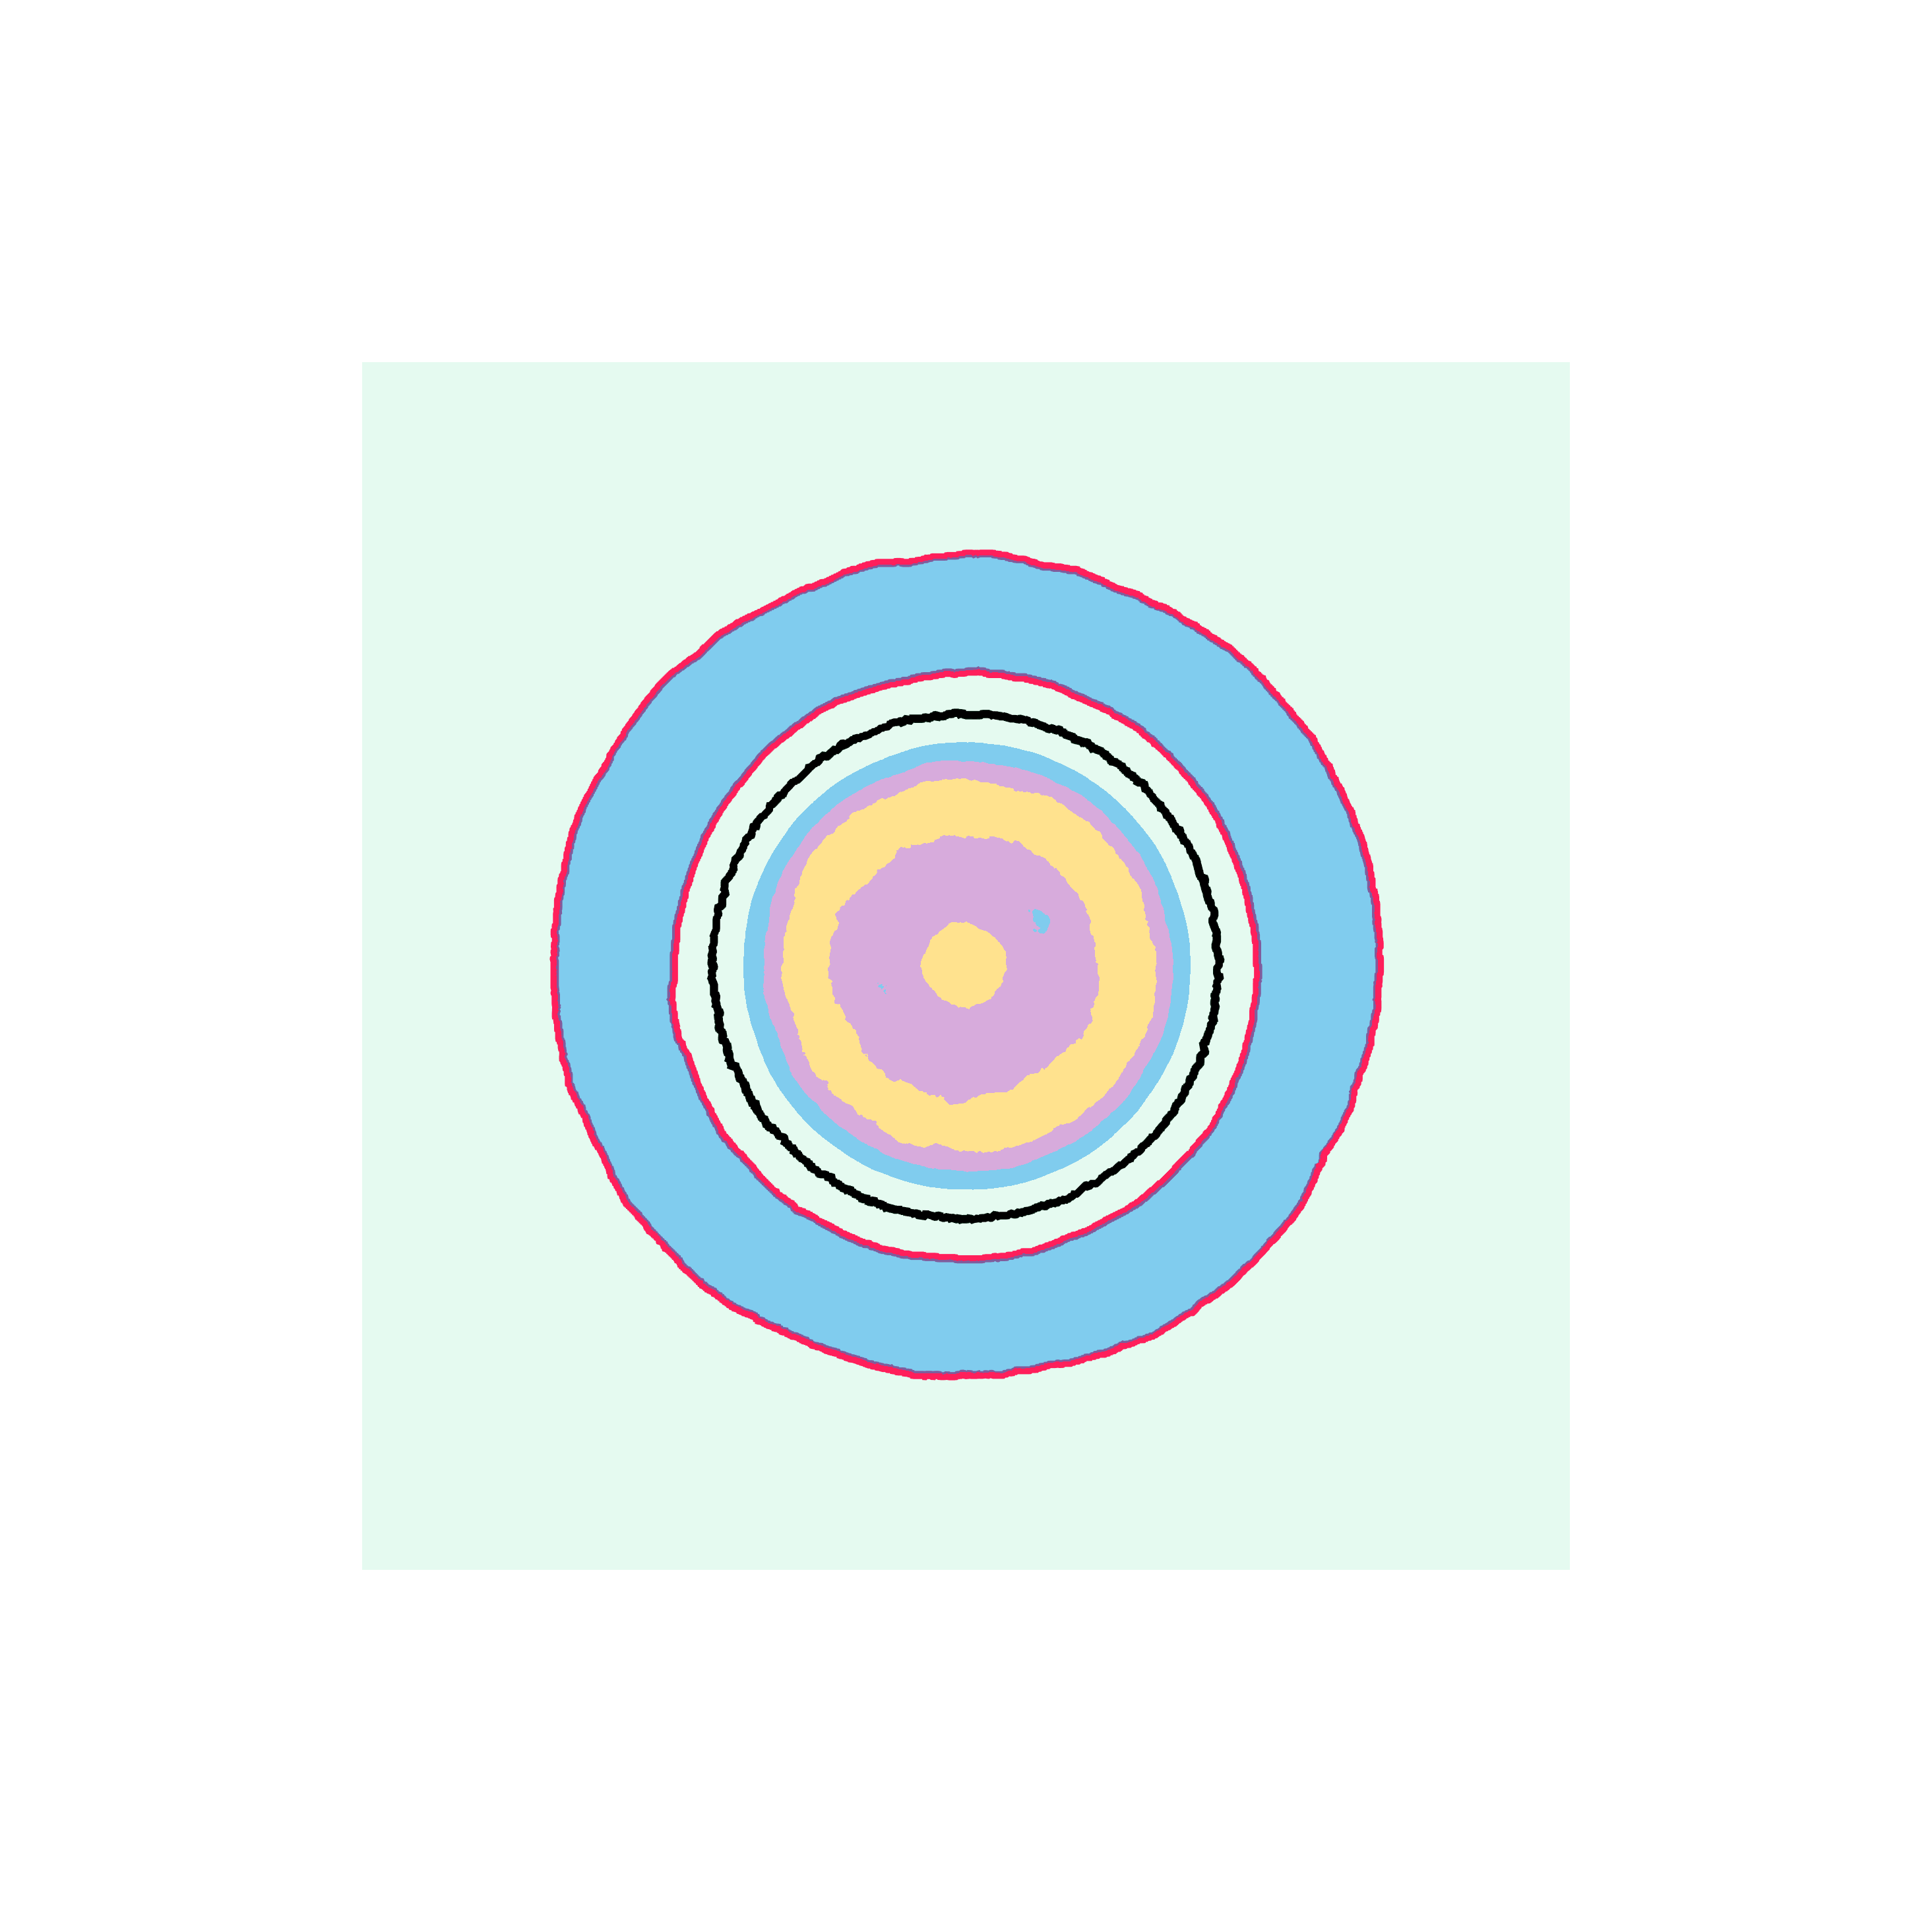
\includegraphics[trim=500 500 500 500, clip, width=0.25\textwidth]{scripts/figures/relative/surf_top-0_0.png}
  % \caption{(Left) Full $\hom_1$ persistence diagram, (middle) $\hom_1$ persistence diagram of the function restricted to the \emph{sub}-levelset $B_{0.3}$, (right) $\hom_2$ persistence diagram of the the function realtive to the sub-levelset $B_{0.3}$.
  \caption{(Top) The indicated infinite features in the restricted and relative diagrams correspond to the birth and death of the 1-feature $(0.18, 0.45)$ in the full diagram.
  (Bottom) In black, the representative cycle of the infinite 1-feature born at 0.18 in the restricted diagram is shown in black.
  In red, the \emph{boundary} of the representative \emph{relative} 2-cycle born at 0.45 in the relative diagram is shown in red.}\label{fig:relative1}
\end{figure}

Now, imagine we obtain the persistence diagram of our sub-levelset $B_\omega$.
That is, we now know that we cover $B_\omega$, or some subset, and do not want to re-compute the diagram above $\omega$.
If we compute the persistence diagram of the function restricted to the \emph{sub}-levelset $B_\omega$ any 1-dimensional features born before $\omega$ that die after $\omega$ will remain infinite features in this restricted (below) diagram.
Indeed, we could match these infinite 1-features with the corresponding shifted finite 1-features in the restricted (above) diagram, as shown in Figure~\ref{fig:restricted}.
However, that would require sorting through all finite features that are born near $\omega$ and deciding if they are in fact features of the full diagram that have been shifted.

Recalling that these same features become infinite 2-features in the relative diagram, we can use the relative diagram instead and match infinite 1-features of the diagram restricted below to infinite 2-features in the relative diagram, as shown in Figures~\ref{fig:relative1} and~\ref{fig:relative2}.
For this example the matching is given by sorting the 1-features by ascending and the 2-features by descending birth time.
How to construct this matching in general, especially in the presence of infinite features in the full diagram, is the subject of future research.

\begin{figure}[htbp]
  \centering
  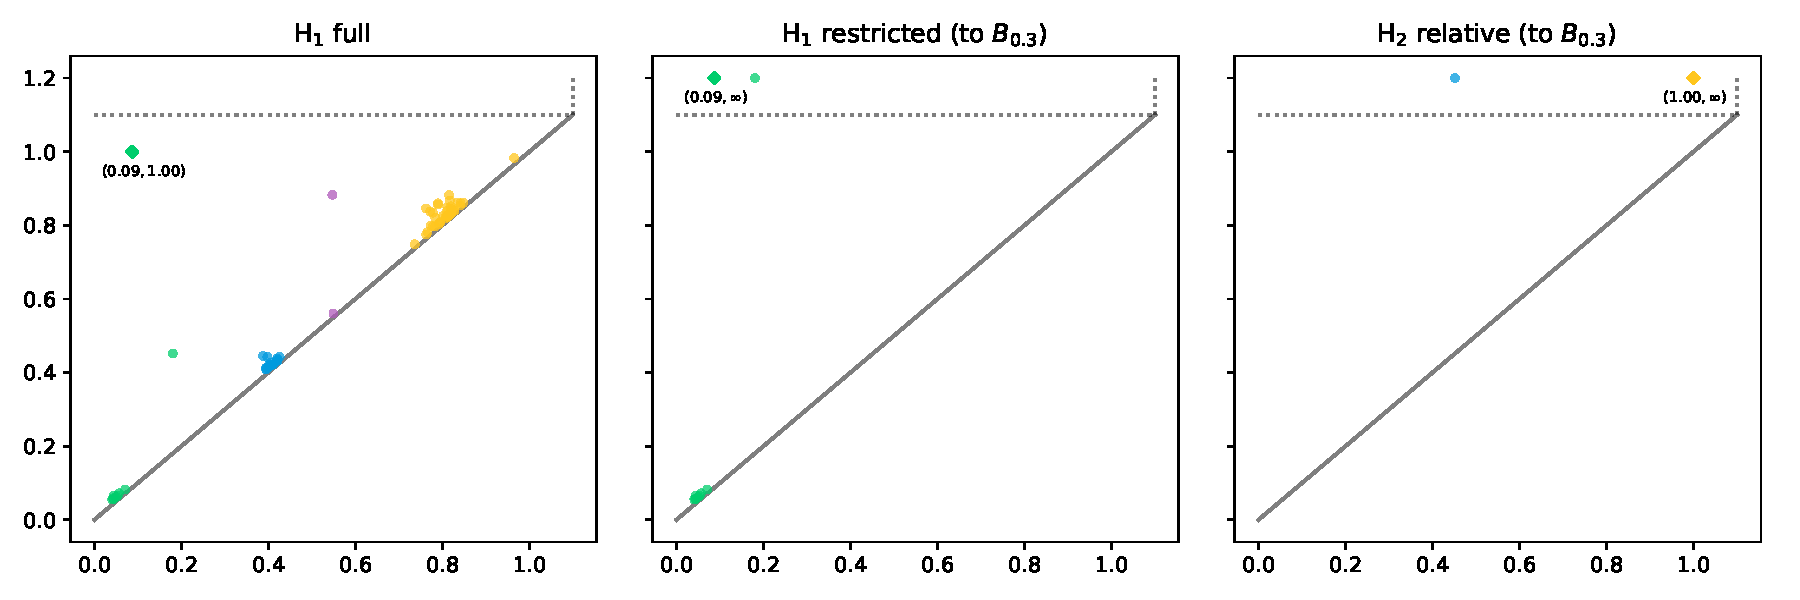
\includegraphics[width=0.9\textwidth]{scripts/figures/relative/dgm-0_1.pdf}
  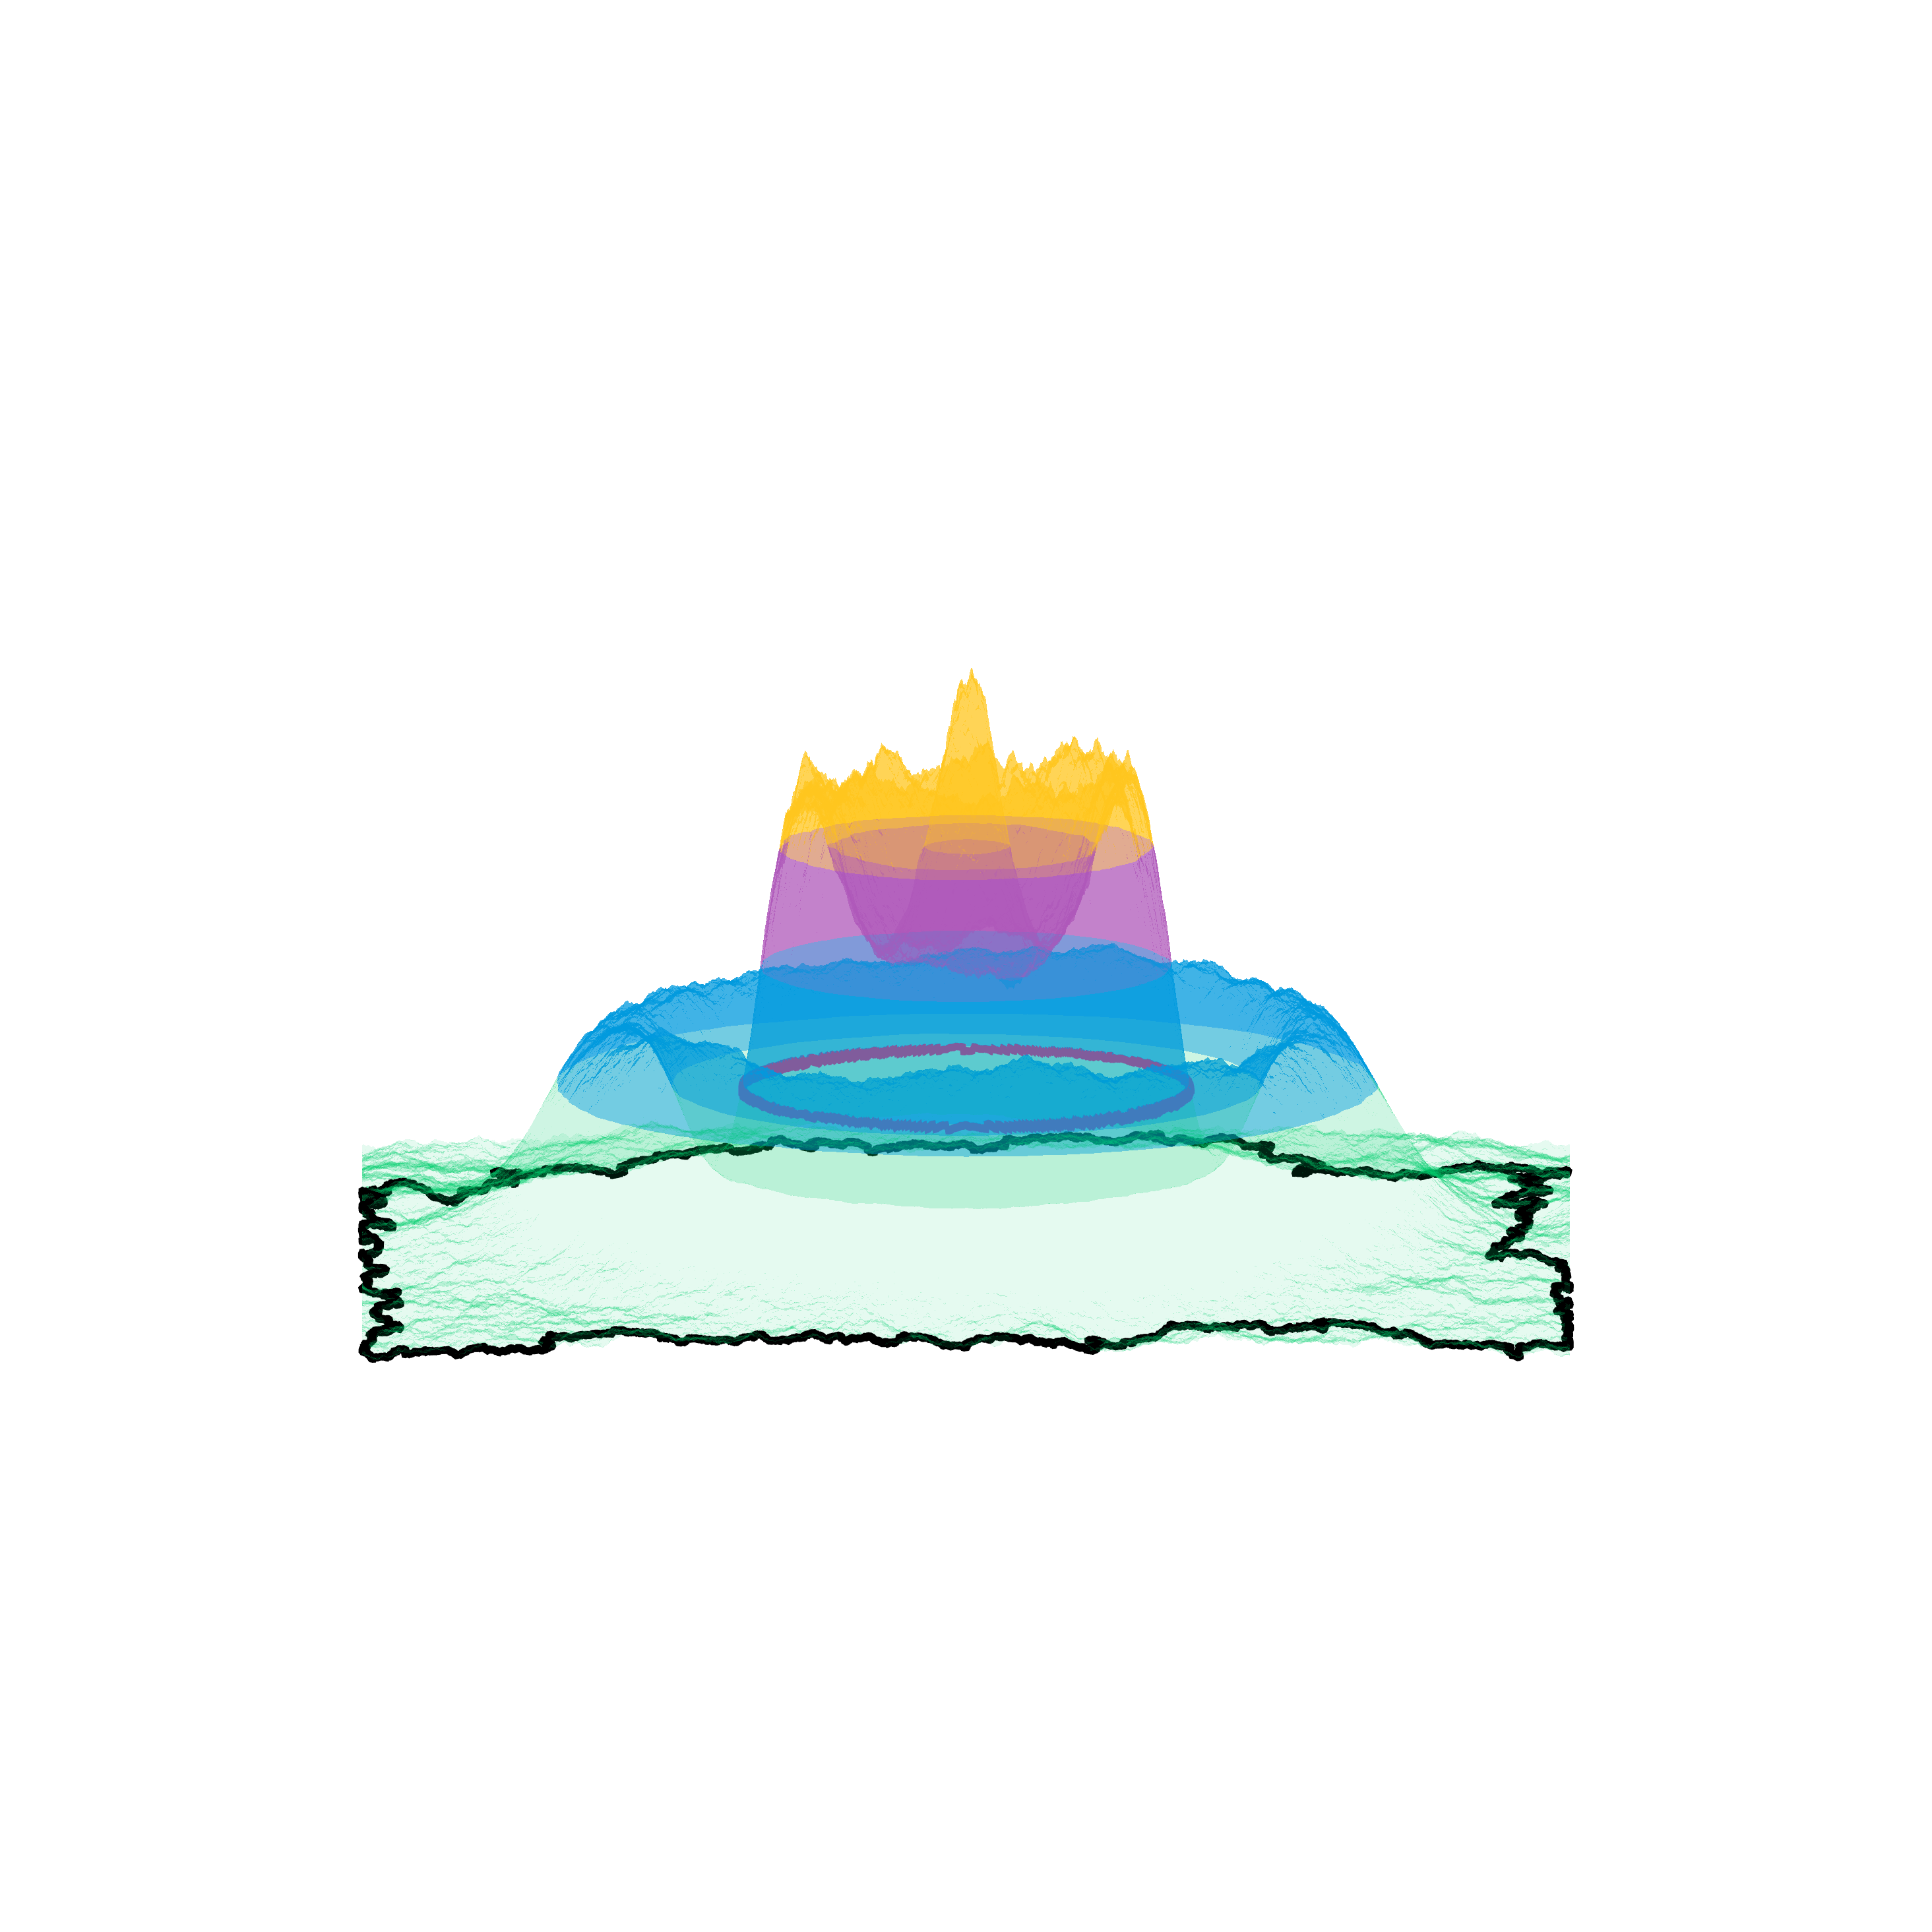
\includegraphics[trim=500 800 500 800, clip, width=0.35\textwidth]{scripts/figures/relative/surf_side-0_1.png}
  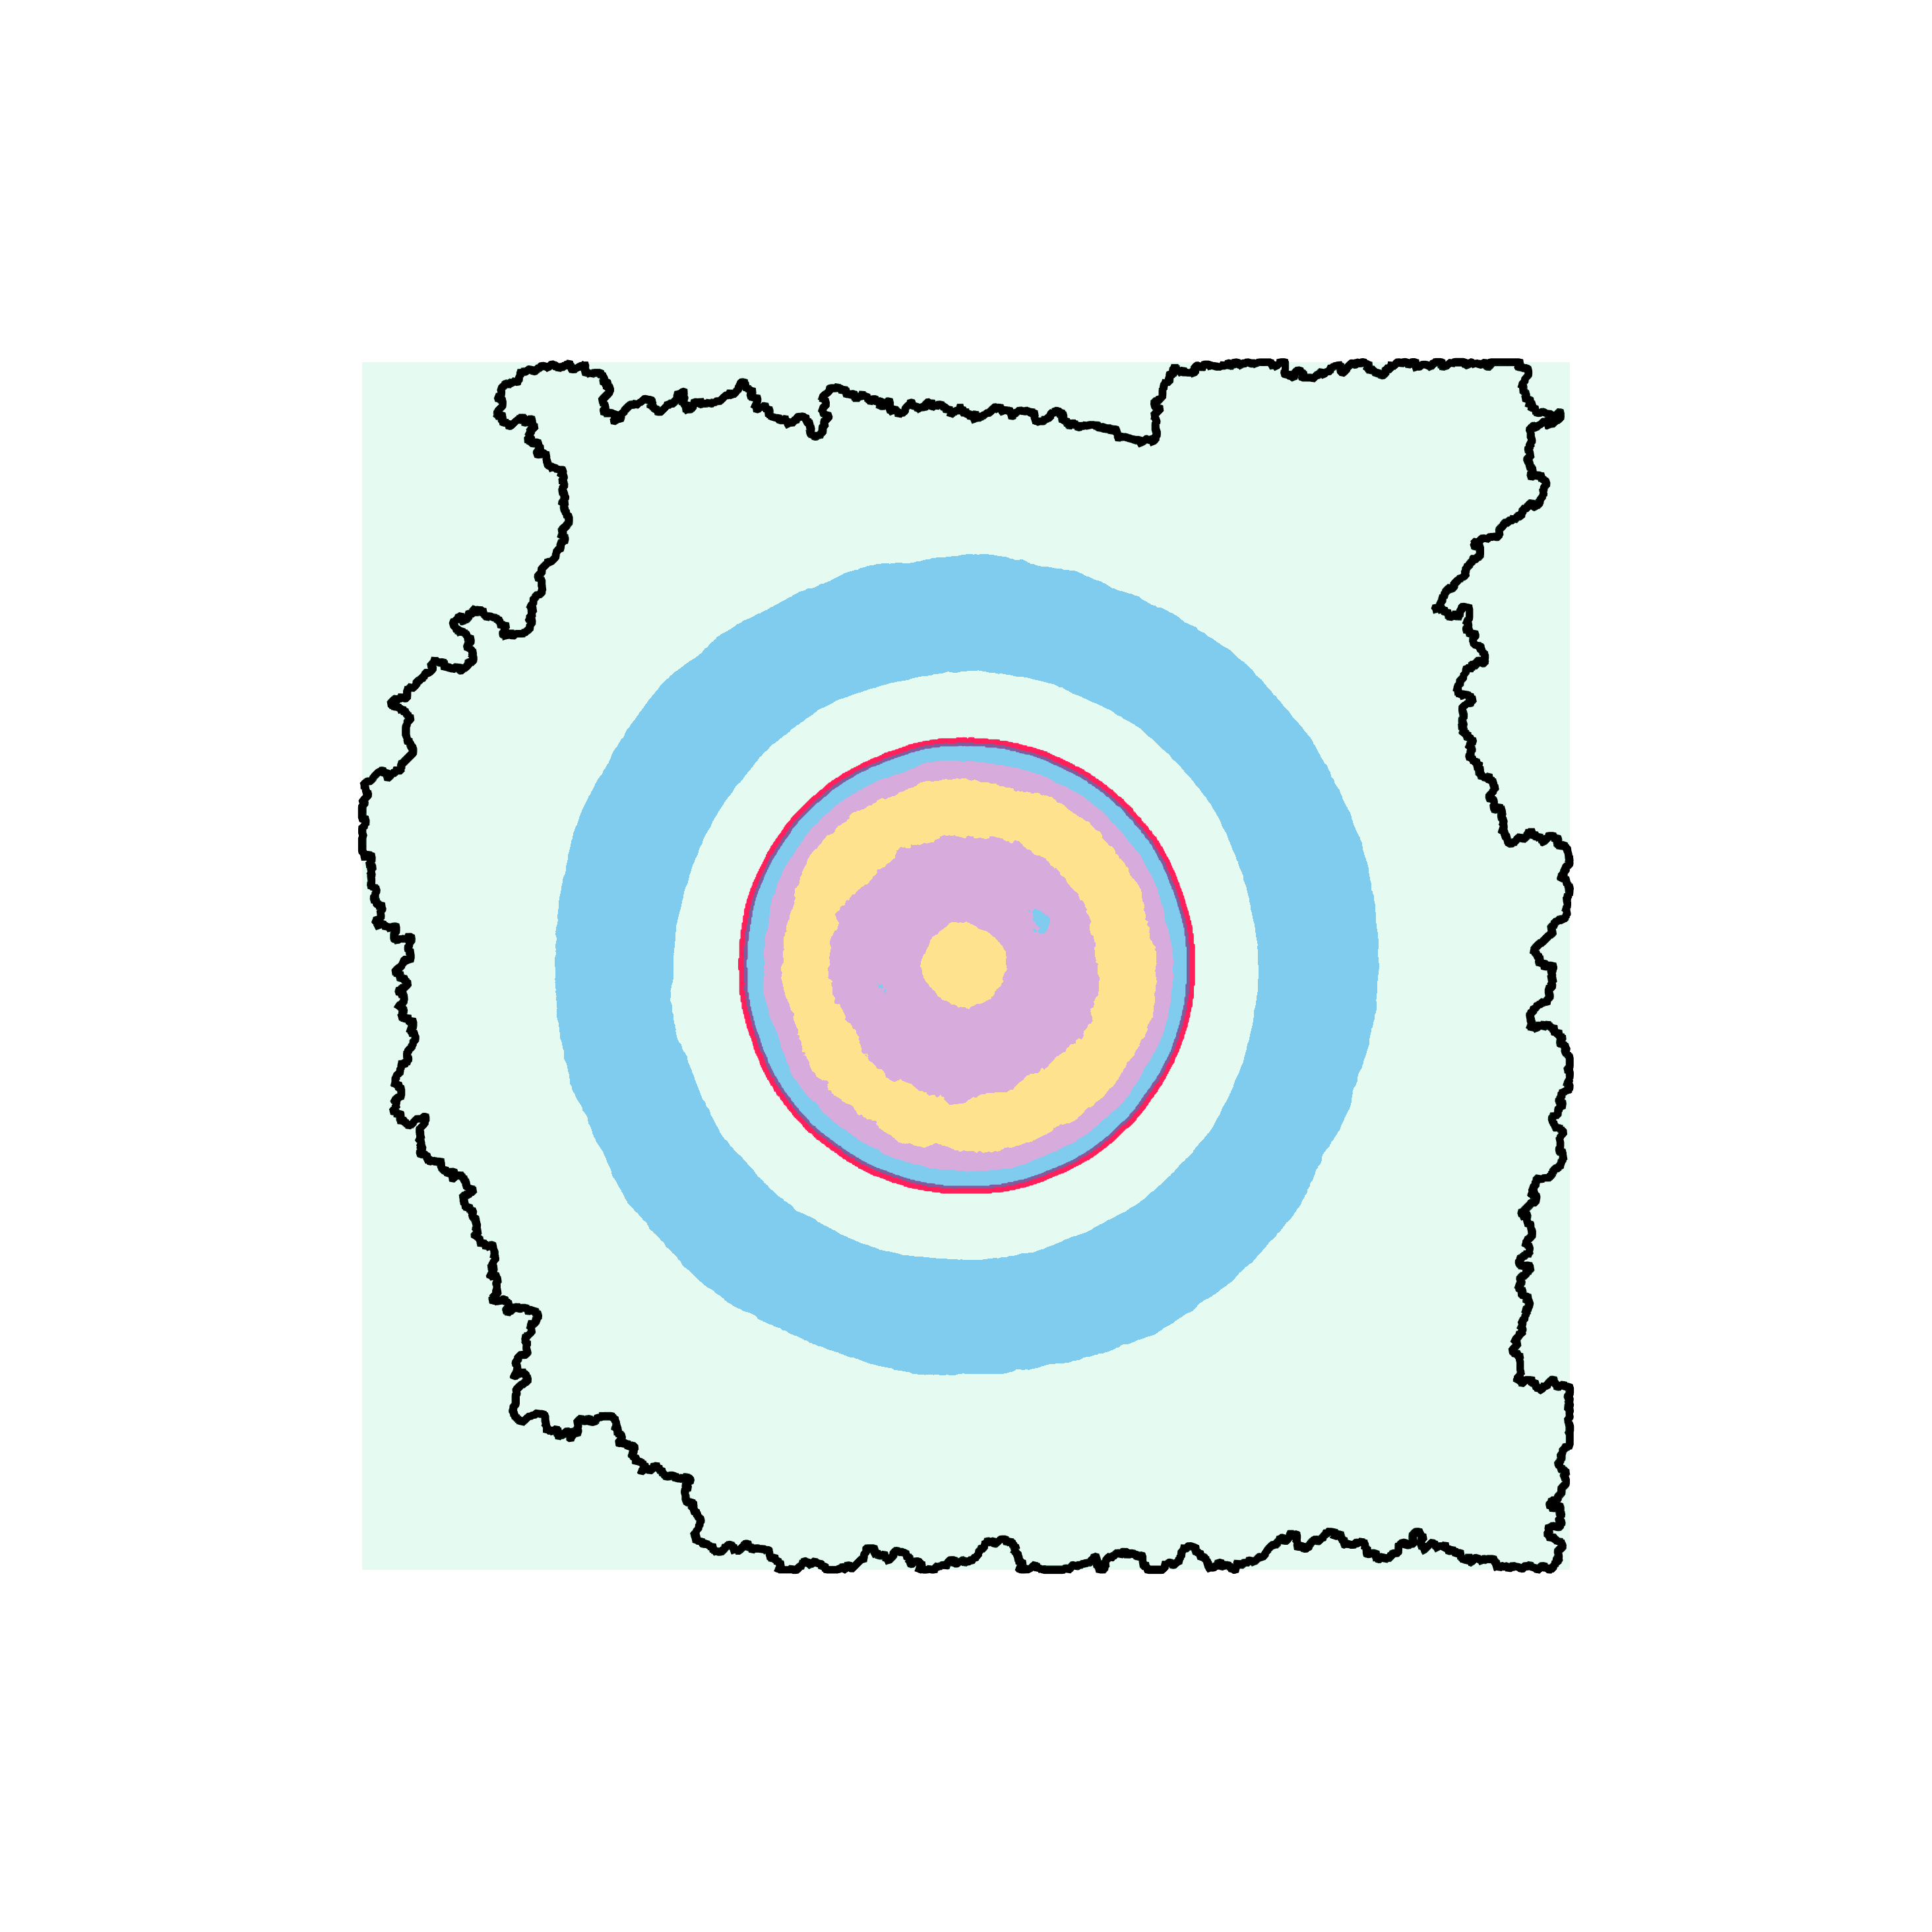
\includegraphics[trim=500 500 500 500, clip, width=0.25\textwidth]{scripts/figures/relative/surf_top-0_1.png}
  \caption{The infinite 1-features of the restricted diagram can be matched with the infinite 2-features of the relative diagrams.
  The sequence birth times of relative 2-features in \emph{decreasing} order correspond to the deaths of restricted 1-features in \emph{increasing} order.}\label{fig:relative2}
\end{figure}
